% Options for packages loaded elsewhere
\PassOptionsToPackage{unicode}{hyperref}
\PassOptionsToPackage{hyphens}{url}
%
\documentclass[
  man,floatsintext]{apa7}
\usepackage{amsmath,amssymb}
\usepackage{iftex}
\ifPDFTeX
  \usepackage[T1]{fontenc}
  \usepackage[utf8]{inputenc}
  \usepackage{textcomp} % provide euro and other symbols
\else % if luatex or xetex
  \usepackage{unicode-math} % this also loads fontspec
  \defaultfontfeatures{Scale=MatchLowercase}
  \defaultfontfeatures[\rmfamily]{Ligatures=TeX,Scale=1}
\fi
\usepackage{lmodern}
\ifPDFTeX\else
  % xetex/luatex font selection
\fi
% Use upquote if available, for straight quotes in verbatim environments
\IfFileExists{upquote.sty}{\usepackage{upquote}}{}
\IfFileExists{microtype.sty}{% use microtype if available
  \usepackage[]{microtype}
  \UseMicrotypeSet[protrusion]{basicmath} % disable protrusion for tt fonts
}{}
\makeatletter
\@ifundefined{KOMAClassName}{% if non-KOMA class
  \IfFileExists{parskip.sty}{%
    \usepackage{parskip}
  }{% else
    \setlength{\parindent}{0pt}
    \setlength{\parskip}{6pt plus 2pt minus 1pt}}
}{% if KOMA class
  \KOMAoptions{parskip=half}}
\makeatother
\usepackage{xcolor}
\usepackage{graphicx}
\makeatletter
\def\maxwidth{\ifdim\Gin@nat@width>\linewidth\linewidth\else\Gin@nat@width\fi}
\def\maxheight{\ifdim\Gin@nat@height>\textheight\textheight\else\Gin@nat@height\fi}
\makeatother
% Scale images if necessary, so that they will not overflow the page
% margins by default, and it is still possible to overwrite the defaults
% using explicit options in \includegraphics[width, height, ...]{}
\setkeys{Gin}{width=\maxwidth,height=\maxheight,keepaspectratio}
% Set default figure placement to htbp
\makeatletter
\def\fps@figure{htbp}
\makeatother
\setlength{\emergencystretch}{3em} % prevent overfull lines
\providecommand{\tightlist}{%
  \setlength{\itemsep}{0pt}\setlength{\parskip}{0pt}}
\setcounter{secnumdepth}{-\maxdimen} % remove section numbering
% Make \paragraph and \subparagraph free-standing
\ifx\paragraph\undefined\else
  \let\oldparagraph\paragraph
  \renewcommand{\paragraph}[1]{\oldparagraph{#1}\mbox{}}
\fi
\ifx\subparagraph\undefined\else
  \let\oldsubparagraph\subparagraph
  \renewcommand{\subparagraph}[1]{\oldsubparagraph{#1}\mbox{}}
\fi
\newlength{\cslhangindent}
\setlength{\cslhangindent}{1.5em}
\newlength{\csllabelwidth}
\setlength{\csllabelwidth}{3em}
\newlength{\cslentryspacingunit} % times entry-spacing
\setlength{\cslentryspacingunit}{\parskip}
\newenvironment{CSLReferences}[2] % #1 hanging-ident, #2 entry spacing
 {% don't indent paragraphs
  \setlength{\parindent}{0pt}
  % turn on hanging indent if param 1 is 1
  \ifodd #1
  \let\oldpar\par
  \def\par{\hangindent=\cslhangindent\oldpar}
  \fi
  % set entry spacing
  \setlength{\parskip}{#2\cslentryspacingunit}
 }%
 {}
\usepackage{calc}
\newcommand{\CSLBlock}[1]{#1\hfill\break}
\newcommand{\CSLLeftMargin}[1]{\parbox[t]{\csllabelwidth}{#1}}
\newcommand{\CSLRightInline}[1]{\parbox[t]{\linewidth - \csllabelwidth}{#1}\break}
\newcommand{\CSLIndent}[1]{\hspace{\cslhangindent}#1}
\ifLuaTeX
\usepackage[bidi=basic]{babel}
\else
\usepackage[bidi=default]{babel}
\fi
\babelprovide[main,import]{english}
% get rid of language-specific shorthands (see #6817):
\let\LanguageShortHands\languageshorthands
\def\languageshorthands#1{}
% Manuscript styling
\usepackage{upgreek}
\captionsetup{font=singlespacing,justification=justified}

% Table formatting
\usepackage{longtable}
\usepackage{lscape}
% \usepackage[counterclockwise]{rotating}   % Landscape page setup for large tables
\usepackage{multirow}		% Table styling
\usepackage{tabularx}		% Control Column width
\usepackage[flushleft]{threeparttable}	% Allows for three part tables with a specified notes section
\usepackage{threeparttablex}            % Lets threeparttable work with longtable

% Create new environments so endfloat can handle them
% \newenvironment{ltable}
%   {\begin{landscape}\centering\begin{threeparttable}}
%   {\end{threeparttable}\end{landscape}}
\newenvironment{lltable}{\begin{landscape}\centering\begin{ThreePartTable}}{\end{ThreePartTable}\end{landscape}}

% Enables adjusting longtable caption width to table width
% Solution found at http://golatex.de/longtable-mit-caption-so-breit-wie-die-tabelle-t15767.html
\makeatletter
\newcommand\LastLTentrywidth{1em}
\newlength\longtablewidth
\setlength{\longtablewidth}{1in}
\newcommand{\getlongtablewidth}{\begingroup \ifcsname LT@\roman{LT@tables}\endcsname \global\longtablewidth=0pt \renewcommand{\LT@entry}[2]{\global\advance\longtablewidth by ##2\relax\gdef\LastLTentrywidth{##2}}\@nameuse{LT@\roman{LT@tables}} \fi \endgroup}

% \setlength{\parindent}{0.5in}
% \setlength{\parskip}{0pt plus 0pt minus 0pt}

% Overwrite redefinition of paragraph and subparagraph by the default LaTeX template
% See https://github.com/crsh/papaja/issues/292
\makeatletter
\renewcommand{\paragraph}{\@startsection{paragraph}{4}{\parindent}%
  {0\baselineskip \@plus 0.2ex \@minus 0.2ex}%
  {-1em}%
  {\normalfont\normalsize\bfseries\itshape\typesectitle}}

\renewcommand{\subparagraph}[1]{\@startsection{subparagraph}{5}{1em}%
  {0\baselineskip \@plus 0.2ex \@minus 0.2ex}%
  {-\z@\relax}%
  {\normalfont\normalsize\itshape\hspace{\parindent}{#1}\textit{\addperi}}{\relax}}
\makeatother

\makeatletter
\usepackage{etoolbox}
\patchcmd{\maketitle}
  {\section{\normalfont\normalsize\abstractname}}
  {\section*{\normalfont\normalsize\abstractname}}
  {}{\typeout{Failed to patch abstract.}}
\patchcmd{\maketitle}
  {\section{\protect\normalfont{\@title}}}
  {\section*{\protect\normalfont{\@title}}}
  {}{\typeout{Failed to patch title.}}
\makeatother

\usepackage{xpatch}
\makeatletter
\xapptocmd\appendix
  {\xapptocmd\section
    {\addcontentsline{toc}{section}{\appendixname\ifoneappendix\else~\theappendix\fi\\: #1}}
    {}{\InnerPatchFailed}%
  }
{}{\PatchFailed}
\keywords{Core threats, Transdiagnostic anxiety, Written Exposure Therapy}
\usepackage{lineno}

\linenumbers
\usepackage{csquotes}
\makeatletter
\renewcommand{\paragraph}{\@startsection{paragraph}{4}{\parindent}%
  {0\baselineskip \@plus 0.2ex \@minus 0.2ex}%
  {-1em}%
  {\normalfont\normalsize\bfseries\typesectitle}}

\renewcommand{\subparagraph}[1]{\@startsection{subparagraph}{5}{1em}%
  {0\baselineskip \@plus 0.2ex \@minus 0.2ex}%
  {-\z@\relax}%
  {\normalfont\normalsize\bfseries\itshape\hspace{\parindent}{#1}\textit{\addperi}}{\relax}}
\makeatother

\ifLuaTeX
  \usepackage{selnolig}  % disable illegal ligatures
\fi
\IfFileExists{bookmark.sty}{\usepackage{bookmark}}{\usepackage{hyperref}}
\IfFileExists{xurl.sty}{\usepackage{xurl}}{} % add URL line breaks if available
\urlstyle{same}
\hypersetup{
  pdftitle={Transdiagnostic Written Exposure Therapy: Piloting an Online Intervention},
  pdfauthor={Elad Zlotnick1, Hila Sorka1, Snir Barzilay1, \& Jonathan D. Huppert1},
  pdflang={en-EN},
  pdfkeywords={Core threats, Transdiagnostic anxiety, Written Exposure Therapy},
  hidelinks,
  pdfcreator={LaTeX via pandoc}}

\title{Transdiagnostic Written Exposure Therapy: Piloting an Online Intervention}
\author{Elad Zlotnick\textsuperscript{1}, Hila Sorka\textsuperscript{1}, Snir Barzilay\textsuperscript{1}, \& Jonathan D. Huppert\textsuperscript{1}}
\date{}


\shorttitle{WET}

\authornote{

This work was supported by\ldots.

The authors made the following contributions. Elad Zlotnick: Conceptualization, Writing - Original Draft Preparation, Writing - Review \& Editing; Hila Sorka: Conceptualization, Writing - Original Draft Preparation, Writing - Review \& Editing; Snir Barzilay: Conceptualization, Writing - Original Draft Preparation, Writing - Review \& Editing; Jonathan D. Huppert: Conceptualization, Writing - Review \& Editing, Supervision.

Correspondence concerning this article should be addressed to Elad Zlotnick, Department of Psychology, The Hebrew University of Jerusalem, Mount Scopus, Jerusalem 91905, Israel. E-mail: \href{mailto:elad.zlotnick@mail.huji.ac.il}{\nolinkurl{elad.zlotnick@mail.huji.ac.il}}

}

\affiliation{\vspace{0.5cm}\textsuperscript{1} The Hebrew University of Jerusalem}

\abstract{%
This is where the abstract goes.
}



\begin{document}
\maketitle

Written interventions have long been part of the psychological toolbox (Ruini \& Mortara, 2022).
They have been used both as an aid and as a central technique (Riordan, 1996; Smyth et al., 2008).
Expressive writing is a therapeutic technique in which individuals freely write about emotional or traumatic experiences (Pennebaker, 1997).
Evidence indicates that expressive writing has a consistent but limited effect (e.g., Frattaroli, 2006).
However, there is evidence that expressive writing is highly effective in specific contexts.
In particular, writing treatments have been found to be effective for PTSD in meta-analyses
(e.g., Emmerik et al., 2013; Gerger et al., 2021) though evidence is mixed (Mogk et al., 2006).

Written Exposure Therapy (WET) is a structured, brief intervention designed to treat traumatic experiences through expressive writing.
Originally developed as a focused application of imaginal exposure (IE), WET was created to offer a streamlined, accessible alternative to more traditional therapies.
Studies have shown that WET yields strong effects, comparable to established treatments like Cognitive Processing Therapy and Prolonged Exposure (Sloan et al., 2012; Sloan et al., 2023; Sloan \& Marx, 2019; Thompson-Hollands et al., 2019).
While WET has traditionally been applied specifically to PTSD, recent studies have extended its use to generalized anxiety (Goldman et al., 2007; Ovanessian et al., 2019) including an online format (Roch-Gagné \& Talbot, 2019), indicating its potential for broader, transdiagnostic applications.

This paper introduces Transdiagnostic WET, a variation of WET tailored for a transdiagnostic population.
Since WET integrates elements of both IE and expressive writing, we address the foundations of each approach to fine-tune Transdiagnostic WET.
Two key insights drive the modifications to WET: exposure needs to be a) focused and b) immersive.

Meta-analyses have found that more directive instructions yield better outcomes in expressive writing (Frattaroli, 2006; Reinhold et al., 2018).
Indeed, WET for PTSD focuses on the most distressing traumatic event that the client has (Sloan \& Marx, 2019).
Furthermore, WET has been found to be more effective when focusing on a single fear rather than alternating between different fears, both in GAD and PTSD (Fracalanza et al., 2014; Sloan et al., 2005).
In PTSD, WET focuses on the central issue of anxiety - the traumatic event - by default .
We propose to improve the focus of WET by explicitly focusing on core threats: the ultimate feared consequence of one's fear or anxiety (Huppert \& Zlotnick, 2012; Zlotnick \& Huppert, 2025).
Clinicians suggest that focusing on core threats in psychological treatments improves efficacy, enhances generalizability, and reduces relapse
(Foa \& Kozak, 1986; Gillihan et al., 2012; Murray et al., 2016).
We have developed an online questionnaire to reliably identify core threats (Zlotnick, 2025).
Thus, to ensure that the intervention is accurately focused, we help participants identify their core threats and then instruct them to focus on these idiosyncratic core threats throughout their writing.

A second set of accommodations to the WET protocol is to help participants create an immersive script.
Building on the work of Lang (1977), emotional processing theory contends that
emotional activation is necessary for emotional processing to occur (Foa et al., 2006; Foa \& Kozak, 1986).
Indeed, IE protocols typically involve conjuring a vivid, detailed image of one's worst case scenario from a first person perspective (e.g., Abramowitz, 2006; Foa et al., 2012).
Furthermore, focusing on the emotional aspects in writing is more beneficial than focusing on cognitive or control conditions (Sloan et al., 2007).
Moreover, individuals undergoing WET show signs of physiological distress, supporting the idea that emotional activation is necessary for successful treatment (Wisco et al., 2016).
However, the WET protocol for PTSD emphasizes recounting traumatic experiences from a distancing perspective (e.g., ``as you look back upon it now'') rather than an immersed perspective (e.g., ``as if it were happening right now;'' Sloan \& Marx, 2019).
This approach is based on the idea that a distanced perspective better facilitates ``working through'' difficult life experiences (Kross \& Ayduk, 2011; e.g., Kross \& Ayduk, 2017).
We argue that this approach is appropriate for PTSD, where a major aspect of the intervention is to reconstruct the traumatic narrative.
Indeed, the WET protocol explicitly states this goal: ``By repeatedly recounting the event, you will be able to correct for the splintered fashion in which the memory may have been stored.'' (Sloan \& Marx, 2019, p. 53).
We contend that for a transdiagnostic, non-traumatized population increased emotional activation is needed.
Thus, we direct participants to immerse themselves in the writing by using first person, providing detailed sensory and emotional descriptions, and periodically closing their eyes and calling upon their imaginations.

The primary goal of this study was to develop and validate the efficacy of future-oriented WET.
However, it is clear that a greater understanding of the underlying mechanisms of interventions will allow more precise interventions (Niv et al., 2021).
Moreover, a holistic theory that integrates their theory is needed (Brewin, 1996; Hofmann \& Hayes, 2019; Huppert et al., 2020).
Thus, we aim to explore several potential mechanisms underlying WET's functioning (cf. Rousseau \& Belleville, 2018).

\textbf{1. Fear reduction:}
Early studies suggested that imaginal exposure promotes habituation of pathological anxiety (e.g., Foa \& Chambless, 1978).
Repeated exposure to the same scenario may lead to fear reduction through habituation---a decreased response to the imagined scenario---or through extinction, wherein the imagined scenario becomes neutral after breaking its association with an aversive stimulus (cf. Cooper et al., 2017).
Fear reduction was assessed through self-reported responses to the imagined scenario before and after the intervention, measured both within and across sessions (see Foa \& Kozak, 1986; Rupp et al., 2017).

\textbf{2. Specific reactions to memories:}
While metacognitive beliefs apply to all mental events, specific memories or images may evoke distinct reactions, such as distress, intrusiveness, or avoidance.
Changes in these reactions may occur without altering broader metacognitive beliefs.
We measured participants' reported reactions to specific memories, assessing changes in distress, intrusiveness, and avoidance.

\textbf{3. Distress tolerance (DTS):}
Distress tolerance has been suggested as a critical factor in the efficacy of exposure therapy, potentially more important than fear reduction itself (Craske et al., 2008; Hayes et al., 1999).
Repeated exposure to intense, negative emotional events may enhance participants' ability to tolerate distress.
We predict that DTS will increase as a result of participants' engagement with the WET protocol.

\textbf{4. Thought fusion:}
The belief that thoughts have direct causal effects on the world, behavior, and objects---referred to as thought fusion---has been linked to intrusive thoughts and OCD as well as other anxiety disorders (Rassin et al., 1999, 2001; Thompson-Hollands et al., 2013).
Exposure to negative imagery without adverse consequences may reduce the perceived importance of thoughts, leading to improved outcomes.
We hypothesize that WET will reduce thought fusion, supporting better symptom management.

\textbf{5. Negative beliefs about images and memories:}
In addition to thought fusion, other metacognitive beliefs about images and memories can maintain distress.
These include beliefs that recalling a memory is dangerous and may lead to losing control, ``going crazy,'' or emotional collapse.
Such beliefs about uncontrollability and danger may perpetuate avoidance and distress.
WET aims to challenge these beliefs by encouraging safe engagement with distressing memories, fostering cognitive restructuring.

This study aims to extend WET in three ways: a) applying it to a transdiagnostic population; b) exploring its utility for coping with anticipated future threats rather than past events; and c) assessing its effectiveness as a self-administered, online intervention.
Our goal is to provide individuals across a transdiagnostic range of anxiety-related disorders with tools to manage anxiety independently.
To date, WET has not been widely tested within this type of sample or setting.
Thus, our primary aim is to evaluate its effectiveness in reducing anxiety symptoms.
We hypothesized that WET will yield greater reductions in anxiety symptoms and improvements in well-being compared to both active control (written distraction imagery) and waitlist control conditions.

An additional aim is to investigate the mechanisms underlying WET's effects, enhancing our understanding of how it facilitates therapeutic change.
More insight into mechanisms could help to fine tune theory, optimize therapeutic processes and improve outcomes (Huppert et al., 2020; Niv et al., 2021).
We measured potential mechanisms that might drive WET's effects, focusing on both threat-specific processes (e.g., fear reduction, reactions to distressing memories) and threat-agnostic processes {[}e.g., distress tolerance, thought fusion, and negative metacognitions regarding memories or images; Rousseau and Belleville (2018){]}.

To explore these processes, we examined whether WET elicits changes in these factors and, if so, whether these changes correlate with reductions in anxiety symptoms.
We anticipate that changes in mechanisms will align with symptom changes, supporting their role in the intervention's therapeutic process.
This experiment was pre-registered prior to data collection \href{https://doi.org/10.17605/OSF.IO/2CEHR}{doi.org/10.17605/OSF.IO/2CEHR}.

\section{Methods}\label{methods}

This study was a randomized controlled trial (RCT) in which participants were randomly assigned to one of two groups: the treatment group (WET) or the control group (Neutral Imagery Writing, NIW).
Additionally, data from a waitlist control group was incorporated, collected from a prior study with the same structure and inclusion/exclusion criteria (see Sorka et al., in preparation).
This provided both a passive control and an active control for comparison.
The study employed a double-blind design to ensure objectivity.
Study personnel had no direct interaction with participants, and both experimenters and participants were unaware of group assignments until the one-week follow-up.
The primary outcome was defined as the change in OASIS scores, with changes in WSAS scores and other proposed mechanisms serving as secondary outcomes.
Covariations between changes in OASIS and changes in each potential mechanism were also explored.

Supplementary materials, including datasets, analysis scripts, and detailed methodological documentation, are available on GitHub at \url{https://github.com/eladzlot/transdiagnostic.wet-2025-public}.
To protect participant confidentiality, the datasets have been redacted to include only quantitative information, as the core threats and other open-ended responses could potentially identify specific individuals.
These resources enhance transparency and facilitate replication of the findings.

\subsection{Participants}\label{participants}

Participants were recruited through the Prolific platform, compensated at \(\pounds 9\)/hour.
Inclusion criteria included high pathological anxiety (greater than 4 on the OASIS),
and impaired daily function (at least one item scored above 2 on WSAS).
Exclusion criteria were severe depression (greater than 14 on the PHQ; Kroenke et al., 2009), post-trauma (greater than 6 on the brief PCL-5; Zuromski et al., 2019), or psychotic symptoms (evaluated via items 19 and 20 from the DIAMOND screener; Tolin et al., 2018).
In addition, English as a fluent language was required.
Furthermore, participants who had reported head injury or reading and writing difficulties in the Prolific system were excluded.
Finally, only experienced users on the Prolific platform with an approval rate of above 95, and with minimum previous submissions of 300 were allowed to participate in this study.
An ethnically diverse sample was requested from Prolific.

A power analysis indicated that a sample size of 148 participants would provide 0.8 power, but due to financial constraints, Bayesian stopping criteria allowed for early termination.
Recruitment continued until region of practical equivalence (ROPE) showed no significant difference could be found between WET and NIW conditions.

Participants were randomly assigned to the treatment and control groups in a 2:1 ratio, using block randomization (\(OASIS \geq 8\)), aiming to ensure equal distribution of anxiety severity between groups.
The randomization process was integrated into the experiment program code.

\subsection{Measures}\label{measures}

The \emph{Overall Anxiety Severity and Impairment Scale} (OASIS; Norman et al., 2006) assesses the frequency, intensity, and functional impairment of anxiety and fear over the past week.
Participants rate their anxiety on a 5-point scale from 0 (little or none) to 4 (extreme or all the time).
Higher scores indicate more severe anxiety-related impairment, with a cut-off score of eight recommended for distinguishing anxiety disorders and a change of four points considered clinically significant (Moore et al., 2015).
The OASIS has strong psychometric properties, with an omega coefficient of 0.86 across timepoints in our sample, indicating high reliability.

The \emph{Work and Social Adjustment Scale} (WSAS; Mundt et al., 2002) was used to assess functional impairment due to anxiety symptoms.
The scale consists of five items, each rated on a 9-point Likert scale (0 = no impairment to 8 = severe impairment), evaluating the extent of difficulty in work, home management, social leisure, private leisure, and close relationships.
In our sample, the omega coefficient was 0.80, indicating high reliability.

The \emph{Thought-Action Fusion Scale Revised} (TAF-R; Shafran et al., 1996) measured the degree to which individuals equate thoughts with actions.
It includes 19 items rated on a 5-point Likert scale (0 = disagree strongly to 4 = agree strongly), with higher scores indicating a stronger tendency toward thought--action fusion.
The scale comprises two subscales: \textbf{TAF-Moral}, which reflects the belief that having unacceptable thoughts is morally equivalent to performing them, and \textbf{TAF-Likelihood}, which captures the belief that thinking certain thoughts increases the likelihood of them occurring.
We analyzed these subscales separately.
In our sample, the omega coefficient for moral and likelihood TAF was 0.94 and 0.97 respectively, indicating excellent reliability.

The \emph{Brief Core Schema Scale} (BCSS; Fowler et al., 2006) was employed to assess positive and negative cognitive self-schemas.
It consists of 24 items regarding the self or others (e.g., ``I am talented''; ``I am loved''), divided into two subscales each (e.g., self-positive and self-negative).
Each item is rated on a 5-point Likert scale (0 = Don't Believe it to 4 = Believe it totally).
In our sample, the omega coefficients for each scale were at least 0.87, indicating excellent reliability.

The \emph{Distress Tolerance Scale} (DTS; Simons \& Gaher, 2005) assessed participants' ability to tolerate distressing emotions and situations.
The DTS consists of 15 items rated on a 5-point Likert scale (1 = strongly agree to 5 = strongly disagree), evaluating various aspects of distress tolerance, including participants' perceived ability to withstand negative emotions without engaging in impulsive behaviors.
Due to a coding mistake, item 6 was missing and item 7 was repeated twice, thus we dropped item 6 completely from all analyses.
In our sample, the omega coefficient was 0.93, indicating excellent reliability.

The \emph{Metacognition Questionnaire-30} (MCQ-30; Wells \& Cartwright-Hatton, 2004) was employed to evaluate metacognitive processes and beliefs related to anxiety.
The MCQ-30 consists of 30 items rated on a Likert scale ranging from 1 (do not agree) to 4 (agree very much).
It assesses five factors of metacognition: cognitive confidence, positive beliefs about worry, cognitive self-consciousness, negative beliefs about the uncontrollability of thoughts and danger, and beliefs about the need to control thoughts.
In our sample, the omega coefficients were at least 0.89, indicating excellent reliability.

The \emph{Self-Compassion Scale-Short Form} (SCS-SF; Raes et al., 2011) assessed participants' levels of self-compassion.
The SCS-SF consists of 12 items rated on a 5-point Likert scale (1 = almost never to 5 = almost always).
Higher scores indicate a greater frequency of self-compassionate thoughts and behaviors.
In our sample, the omega coefficient was 0.85, indicating excellent reliability.

The \emph{Impact of Future Event Scale} (IFES; Deeprose et al., 2011) assessed the impact of intrusive prospective, personally-relevant imagery.
Participants completed 24 items evaluating intrusive pre-experiencing, avoidance, and hyper-arousal, responding to how frequently each statement was true for them over the past seven days.
Responses were given on a 5-point scale (0 = not at all to 4 = frequently).
For example, one item asked, ``Pictures about the future popped into my mind.''
In our sample, the omega coefficient was 0.89, indicating excellent reliability.

The \emph{Brief State Anxiety Measure} (BSAM; Berg et al., 1998) was used to assess participants' state anxiety in response to their core threat.
The BSAM consists of six items (relaxed, steady, strained, comfortable, worried, tense) adapted from the State-Trait Anxiety Inventory (STAI).
These items are designed to provide a brief and efficient measure of state anxiety.
Each item is rated on a 7-point scale (1 = Not at all, 4 = Very much so), with higher scores indicating greater levels of anxiety.
In this study, participants were asked to imagine their core threat script for a few moments both before and after each writing session.
They then completed the BSAM to report their current anxiety levels.
The BSAM demonstrated excellent internal consistency in our sample, as indicated by an omega coefficient of 0.96.

The \emph{Treatment Credibility Questionnaire} (Devilly \& Borkovec, 2000) was used to evaluate treatment credibility.
Credibility was assessed once, at the middle of Session 1, following the presentation of the overall treatment rationale and before the intervention itself.
Patients rated the therapy on a scale from 0 (not at all) to 8 (very), assessing both how they felt about the intervention and how effective they believed it would be.
The scale has demonstrated strong internal consistency and test--retest reliability (Devilly \& Borkovec, 2000).

\subsection{Procedure}\label{procedure}

The final protocol consists of several steps.
In the initial phase, participants identified and articulated their core threats, which represent the ultimate fears underlying their anxiety.
They then developed a concise script connecting proximal threats to core threats, creating a clear narrative of how these threats were expected to unfold.
Participants engaged in four 20-minute writing sessions designed to facilitate emotional processing, followed by two follow-up sessions: the first one week after completing the intervention and the second two months later (see Figure \ref{fig:progress}).
Outcomes were measured at each session, while mechanisms were assessed pre- and post-intervention to observe the dynamics of change (see Kazdin, 2007).



\begin{figure}
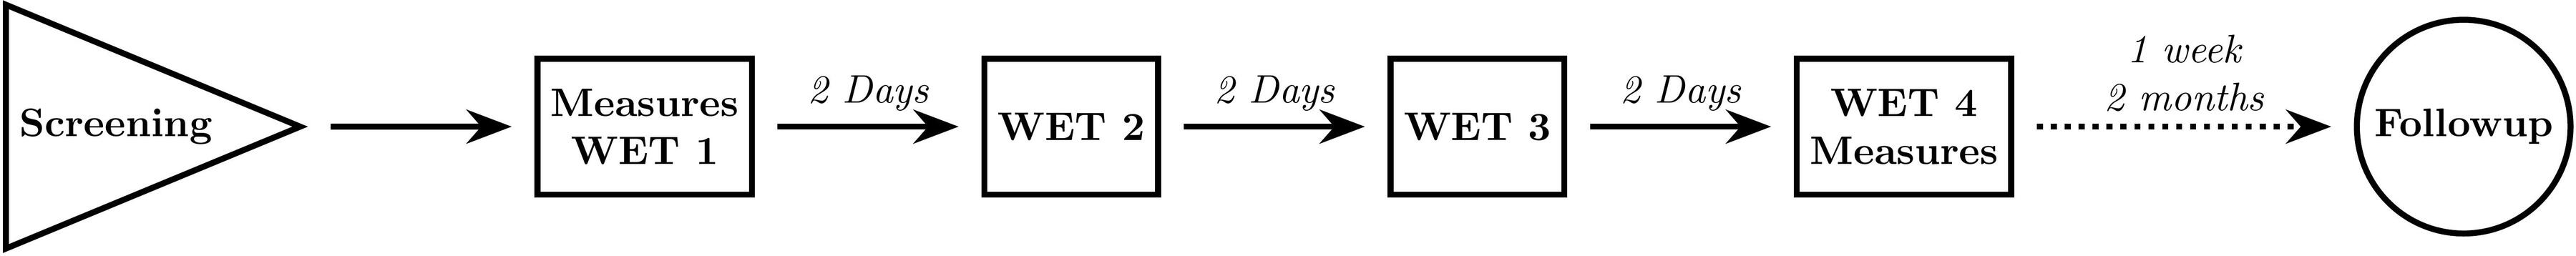
\includegraphics[width=1\linewidth]{../images/progress-resized} \caption{The timeline of the experiment. WET stands for writing for both WET and NIW groups. The waitlist control group completed the questionnaires at time equivalent to WET 1, WET 4, and the 1 week follow-up}\label{fig:progress}
\end{figure}

Symptoms, measured using the OASIS, were assessed before each writing session, except for the final session, where symptoms were measured after writing.
Additionally, symptoms were measured at both follow-up sessions.
Functioning, measured using the WSAS, was assessed at pre-intervention, post-intervention, and both follow-ups.
Mechanisms were evaluated at pre-intervention (before the first writing session) and post-intervention (after the fourth writing session).

Participants were divided into three groups: WET, NIW, and waitlist.
The WET group was instructed to expand on their threat script, focusing on repeated and detailed exposure to distressing content, while the NIW group was guided to identify and describe a neutral situation emphasizing sensory details without emotional valence.
Both groups were instructed to write vividly and in detail, describing their thoughts and emotions during the exercise.
The WET group received standard exposure-based psychoeducation, which emphasized how confronting distressing material could reduce emotional impact over time.
In contrast, the NIW group received psychoeducation highlighting the value of distraction and mental control in fostering emotional regulation.
The waitlist group, which served as a control, completed the OASIS and WSAS three times at one-week intervals to mirror the timepoints of pre-intervention, post-intervention, and one-week follow-up.
Full instructions for both WET and NIW, including psychoeducation materials, are available in the supplementary materials.

\subsection{Statistical Analysis}\label{statistical-analysis}

\subsubsection{Change Model}\label{change-model}

In this study, we employ a multilevel ANCOVA design to account for the nested structure of the data, where anxiety responses are measured repeatedly within individuals over time (Bodner \& Bliese, 2018; van Breukelen, 2013).
The data collected is hierarchical in nature, with multiple measurements nested within each individual.
This nested structure can lead to dependencies among observations within the same individual, violating the assumption of independence in traditional ANCOVA.
For example, rate of change during the treatment is likely correlated to baseline symptom levels.
Multilevel modeling, addresses these dependencies by incorporating random effects to capture the variability within and between individuals.
By accounting for both within- and between-subject variability, multilevel modeling reduces bias that could arise from unaccounted dependencies in repeated measures, thus providing more precise estimates of the treatment effects.
Furthermore, it becomes possible to investigate individual as well as group level effects (Raudenbush \& Bryk, 2002).

To understand change, the estimand is the group level rate of change at each time point.
In the first part of the study, efficacy was examined by the \emph{fixed effects} --- the average rates of change across individuals.
These fixed effects allow us to assess the overall population-level impact of the interventions on anxiety symptoms and mechanisms at different time points.

In the second part of the study, symptom-mechanisms covariation was examined by modeling the \emph{random effects} --- the individual deviations from the group-level trends.
These random effects allow us to capture individual differences in rates of change and explore how these differences relate to the proposed change-driving mechanisms.
By modeling both fixed and random effects, we can explore not only the general efficacy of the intervention but also the individual variability in response to treatment, which may reveal underlying mechanisms.

To account for follow-up measurements at varying time lags (e.g., 1 week, 2 months), we employ a \textbf{piecewise growth model}, allowing for separate slopes at different follow-up times (Andersson et al., 2013; Bollen \& Curran, 2006).
This model enables us to estimate distinct rates of change during different phases of the study.
Combined with the measurement model described below, this is in essence a latent change score model (Cáncer et al., 2021; McArdle, 2009).

The equation for this linear model is as follows:

\[\theta_{ti} = \beta_{0i} + \beta_{1i} \cdot \min(t-1, 3) \cdot 1_{\{t > 1\}} + \beta_{2i} \cdot 1_{\{t > 5\}} + \beta_{3i} \cdot 1_{\{t=6\}}\]
\[\beta_{ji} = \bar{\beta}_{j,\text{condition}} + u_{ji}\]

The latent symptom severity (\(\theta\)) is linearly modeled as a baseline effect (\(\beta_{0i}\)) for each individual and the rate of change after the first session and up to the fourth session (\(\beta_{1i}\)).
Separate terms (\(\beta_{2i}\)) and (\(\beta_{3i}\)) represent the rate of change at follow-up (1 week, 2 months), allowing for flexible modeling of changes at different time intervals.
The individual-specific effects, (\(\beta_{ji}\)), are modeled as deviations from the group-level effects, (\(\bar{\beta}_{j,\text{condition}}\)), to capture both individual and group variability.

\subsubsection{Measurement Model}\label{measurement-model}

Given that anxiety was measured using an ordinal scale, we linked latent symptom severity (\(\theta\)) to the observed ordinal responses using an ordered logit model with a cumulative link function (McCullagh, 1980).
This model assumes that ordinal responses are generated by an underlying continuous latent variable, with thresholds (\(\kappa\)) defining the response categories.
The ordered logit function estimates the probability (\(\phi\)) of endorsing each response category based on the latent symptom severity trait (\(\theta\)).

To account for measurement error and the multidimensionality of the anxiety construct, we adopted a graded response model (GRM) from the item response theory (IRT) framework (Samejima, 2016).
The GRM is well-suited for ordinal data, modeling the probability of endorsing an item category as a function of both item-specific parameters (discrimination: (\(\alpha\)), and difficulty: (\(\beta\)) and the individual's latent trait level (\(\theta\)).

The GRM allows us to model the latent symptom severity (\(\theta\)) for each individual at a specific time point, while accounting for the unique characteristics of each item.
The discrimination parameter (\(\alpha\)) captures how well each item distinguishes between individuals with different levels of anxiety, while the difficulty parameter (\(\beta\)) reflects the trait level required to endorse higher response categories.
This approach helps address known issues with the reliability of change scores (Prieler \& Raven, 2008; Rodebaugh et al., 2016).

In this framework, \(\theta\) is estimated from the multilevel model described earlier, capturing both individual-specific (random) effects and group-level (fixed) effects.
The integration of the GRM with the broader multilevel model allows us to model the latent trait accurately, taking into account both item-level variability and individual differences in anxiety over time.

The equation for the measurement model is as follows:

\[R_{itq} \sim \text{Ordered-logit}(\phi_{itq}, \kappa)\]
\[\phi_{itq} = \alpha_q \cdot (\theta_{it} - \beta_q)\]

Here, the likelihood function represents the probability of observing the ordinal response (\(R\)), given the latent symptom severity (\(\theta\)).
The IRT model specifies the relationship between the latent trait and the item parameters, providing a comprehensive approach to modeling anxiety across individuals.
Detailed specifications for this model are provided in Appendix 1, and the full code is available in the supplementary materials.

\subsection{Mechanisms}\label{mechanisms}

Our second research question investigates the role of various mechanisms in driving changes in pathological anxiety.
While establishing causality is notoriously difficult, particularly in psychological research (Eronen, 2020), our goal is to identify correlations that may signal possible causal relationships.

Mechanisms of change in psychotherapy refer to the processes or events through which psychological interventions achieve their effects on symptoms or functioning.
Demonstrating that an intervention causes a change, does not explain \emph{why} these changes came about.
Establishing a mechanism requires strong association between the treatment and process, and between the process and the outcome (Kazdin, 2007).
Thus, our task is to establish an association between the process and outcome for each process that was found to change by the treatment.

The question here focuses on the process of change, thus we're interested in an association between \emph{changes} in process and mechanism.
We use multivariate latent curve models to examine the association between symptoms and process as they change through time (Baldwin et al., 2014; Damian, 2010; MacCallum et al., 1997).
This approach extends common univariate growth models by allowing the simultaneous examination of multiple outcomes, capturing both the relationships between individual processes and how they evolve over time.
Specifically, we model both anxiety (as measured by the OASIS) and the process of interest in parallel, using a single covariance matrix to estimate the random effects for both processes.
Detailed specifications for this model are provided in Appendix 2, and the full code is available in the supplementary materials.

By incorporating a shared covariance matrix, we capture the correlations between baseline values (intercepts) and changes (slopes) both within and across the two outcomes.
This enables us to test whether baseline levels of a mechanism predict changes in anxiety (moderation) and whether changes in the mechanism correlate with changes in anxiety (mediation).
These cross-process correlations help identify which mechanisms are most strongly associated with changes in anxiety, guiding future research aimed at testing causal pathways.

Although this analysis does not establish causality, it offers valuable insights into potential intervention targets.
For example, identifying mechanisms that strongly correlate with changes in anxiety could inform more focused treatments by highlighting which processes to target for clinical improvement.
Further research will need to extend these findings by extending them into full mediation models (Hilley \& O'Rourke, 2022).

\subsubsection{Missing Data and Estimation}\label{missing-data-and-estimation}

All participants who began the intervention were included in the analysis.
Missing data were imputed via Bayesian imputation, assuming that missingness may be affected by baseline trait levels and task completion difficulty.

We used Bayesian methods to estimate the parameters of the model using Markov Chain Monte Carlo (MCMC) algorithms implemented in Stan (Carpenter et al., 2017), and via the rethinking interface (McElreath, 2020).
We specified weakly informative priors for the regression coefficients, the thresholds, and the item parameters.
We assessed the convergence and the fit of the model using posterior predictive checks, trace plots, and effective sample sizes.
We use a credible interval of 89\% (McElreath, 2020).

\section{Results}\label{results}

\subsection{Participants}\label{participants-1}

Recruitment began August 6, 2023, and ended September 25, 2023, and the final assessment occurred December 2, 2023.
Of 375 individuals initially screened,
89 were randomly assigned at a 2:1 ratio to WET (n = 60, 67.4\%) or NIW (n = 29, 32.6\%) conditions.
The age of participants in the NIW group was significantly lower than that of participants in the WET group (Wilcoxon test, \(W = 628.00\), \(p = .044\)).
Fisher exact test indicated no significant group differences in ethnicity or sex, and Wilcoxon tests showed no significant group differences for pre-treatment symptom measures (\(ps >\) 0.36).

Given the similarity in post-treatment outcomes between the treatment and control groups, we incorporated additional data (n = 73) from a waitlist control group.
This data was collected in a similar study conducted between February 1 and February 24, 2023 (Sorka et al., in preparation).
This was done in order to make sure that the changes found during the intervention were not due to chance.
These subjects were randomly assigned to a waitlist control group for a study that focused on mechanisms of imagery rescripting.
Given the identical inclusion/exclusion criteria and the minor time gap between data collection periods, we expect no systematic differences between the groups.
The CONSORT flowchart (see Figure \ref{fig:consort}) provides a detailed overview of the recruitment, randomization, and follow-up processes across the two active groups.



\begin{figure}
\includegraphics[width=1\linewidth]{/home/eladzlot/projects/wet/docs/output/wet_files/figure-latex/consort-1} \caption{A CONSORT flowchart providing a detailed overview of the recruitment, randomization, and follow-up processes across the two active groups.}\label{fig:consort}
\end{figure}

The large majority of participants (n = 73, 82.0\%) completed all assessments.
Study completion rates did not differ between treatment (81.7\%) and control (82.8\%); Fisher's exact test, \(p\) \textgreater{} .999.
Female participants had a significantly lower attrition rate (11.5\%) compared to males (32.1\%); Fisher's exact test, \(p\) = 0.034.
Fisher's exact and Wilcoxon tests revealed no significant differences between study completers and non-completers in terms of age, ethnicity, or symptom measures (\(ps > 0.24\)).
A detailed breakdown of pre-treatment demographic and symptom characteristics can be found in Table 1.



\begin{table}[tbp]

\begin{center}
\begin{threeparttable}

\caption{\label{tab:demographics}Pre-treatment and Demographic Characteristics of Intent-to-Treat Sample. WET = Written Exposure, NIW = Neutral Imagery Writing, Waitlist group were added as a reference from a different study (Sorka et al., in preparation).}

\begin{tabular}{lllll}
\toprule
 & \multicolumn{2}{c}{Conditions}  &\\
\cmidrule(r){2-4}
Characteristics & NIW & WET & Waitlist & Total\\
\midrule
N & 29 & 60 & 73 & 162\\
Age M (SD) & 36 (11.9) & 42.6 (15.3) & 42.6 (13) & 41.4 (13.8)\\
Gender Female & 22 (75.9\%) & 39 (65\%) & 48 (65.8\%) & 109 (67.3\%)\\
Gender Male & 7 (24.1\%) & 21 (35\%) & 25 (34.2\%) & 53 (32.7\%)\\
Ethnicity &  &  &  & \\
\ \ \ Asian & 3 (10.3\%) & 7 (11.7\%) & 3 (4.1\%) & 13 (8\%)\\
\ \ \ Black & 4 (13.8\%) & 2 (3.3\%) & 1 (1.4\%) & 7 (4.3\%)\\
\ \ \ White & 22 (75.9\%) & 51 (85\%) & 69 (94.5\%) & 142 (87.7\%)\\
Outcomes &  &  &  & \\
\ \ \ OASIS M (SD) & 8.3 (3) & 7.6 (2.7) & 7.8 (2.8) & 7.8 (2.8)\\
\ \ \ WSAS M (SD) & 15.3 (6.8) & 12.5 (6.4) & 12.5 (6.4) & 13 (6.5)\\
\bottomrule
\addlinespace
\end{tabular}

\begin{tablenotes}[para]
\normalsize{\textit{Note.} Data are presented as number (percentage) of patients unless otherwise indicated.}
\end{tablenotes}

\end{threeparttable}
\end{center}

\end{table}

\subsection{Intervention Quality}\label{intervention-quality}

Both WET and NIW were rated highly on the Devilly Credibility Scale, indicating strong credibility in both interventions.
On the cognitive subscale, WET scored 20.0 (6.5), while NIW scored 20.5 (7.1).
Similarly, on the feeling subscale, WET scored 8.7 (3.8) and NIW scored 9.4 (4.1).
These results suggest that participants found both interventions to be highly credible in terms of both their perceived logic and their intuitive appeal.

Participants generally found the writing task acceptable, though some in the WET condition reported it as difficult, while some in the NIW condition described it as progressively boring.

Participants in the WET condition successfully created powerful exposure scripts that addressed their core threats.
For instance, an excerpt from the script of a socially anxious individual reads:

\begin{quote}
What am I doing here? I am a nobody. I know nothing. I feel almost sick now with nerves and dread. What if I just left now? Would anyone even notice? But it's too late\ldots{}\\
I am to speak first, so I can't even steal other people's ideas\ldots{}\\
{[}They're thinking{]} Who is this idiot? I stumble on and on. I want to stop and for it all to be over, but I can't. It just goes on forever. It is like dying in slow motion.
\end{quote}

Adherence in the NIW condition was less strict, with some participants writing scripts that focused on positive outcomes rather than neutral events.
For example, one participant wrote:

\begin{quote}
I feel enthusiastic about starting my day on a positive and productive day.
Today instead of going through my phone for an hour on social media, I start with making my bed and cleaning my room.
\ldots{} I start applying for opportunities that align with my qualifications and a bit of me is worried but still hopeful that I get recognized and recruited.
\end{quote}

This type of writing is similar to what is done in imagery rehearsal (cf. Krakow \& Zadra, 2006).

\subsection{Symptom Measures}\label{symptom-measures}

We fit a Bayesian latent growth curve model to assess the efficacy of the interventions (see Figure \ref{fig:growth} for a visualization of the model's estimated trajectories).
We calculated the standardized mean change (SMC) for each group using the pre-treatment standard deviation as the denominator (Becker, 1988).
This standardization allows comparisons across measures, with higher effect size values indicating better outcomes.
Additionally, we report the probability of direction, which quantifies the certainty that the outcome is greater than 0.
The probability of direction, marked in this paper as P(\textgreater0), ranges from 0 to 1, where values close to 0 indicate high certainty of a negative effect (symptom deterioration), and values close to 1 indicate high certainty of a positive effect (symptom improvement See Makowski et al., 2019).



\begin{figure}
\centering
\includegraphics{/home/eladzlot/projects/wet/docs/output/wet_files/figure-latex/growth-1.pdf}
\caption{\label{fig:growth}Estimated treatment trajectories for each intervention based on the latent growth model. Values are adjusted for gender. WET = Written Exposure Therapy; NIW = Neutral Imagery Writing. The time intervals between pre-treatment and post-treatment, and between post-treatment and followup 1 (FU1), were approximately one week. The interval between FU1 and followup 2 (FU2) was approximately two months, which is indicated by the dashed regression line. The shaded gray area represents the 89\% credible interval (CI).}
\end{figure}

Trait anxiety, as measured by the OASIS, significantly improved across all three interventions at the one-week follow-up.
The estimated raw score improvements were M = 2.73, 89\% CI {[}2.14, 3.35{]}, P(\textgreater0) = 100\% for the WET group, M = 2.59, 89\% CI {[}1.74, 3.41{]}, P(\textgreater0) = 100\% for the NIW group, and M = 0.86, 89\% CI {[}0.23, 1.45{]}, P(\textgreater0) = 98\% for the Waitlist group.

Participants in the WET group showed significant improvements during the treatment period compared to the Waitlist group (\emph{d} = 0.35, 89\% CI {[}0.09, 0.62{]}, P(\textgreater0) = 99\%).
These gains continued at a similar rate at the one-week follow-up, again compared to the Waitlist group (\emph{d} = 0.34, 89\% CI {[}0.13, 0.56{]}, P(\textgreater0) = 99\%).
At the two-month follow-up, the gains were likely continued at a slower rate relative to the projected Waitlist trajectory, as no Waitlist data was collected at this time point (\emph{d} = 0.16, 89\% CI {[}-0.23, 0.57{]}, P(\textgreater0) = 74\%).
The improvement trajectory appeared linear, with consistent gains observed throughout the intervention and continuing during both follow-ups.
Total improvement when compared to the projected Waitlist trend was \emph{d} = 0.85, 89\% CI {[}0.37, 1.37{]}, P(\textgreater0) = 100\%.

Participants in the NIW group also demonstrated significant improvements during the treatment period compared to the Waitlist group (\emph{d} = 0.47, 89\% CI {[}0.18, 0.76{]}, P(\textgreater0) = 100\%).
These improvements were sustained at the one-week follow-up, again in comparison to the Waitlist group (\emph{d} = 0.09, 89\% CI {[}-0.14, 0.33{]}, P(\textgreater0) = 73\%).
At the two-month follow-up, the gains were maintained relative to the projected Waitlist trajectory, as no Waitlist data was collected at this time point (\emph{d} = -0.03, 89\% CI {[}-0.44, 0.38{]}, P(\textgreater0) = 43\%).
Although participants in the NIW group showed considerable overall improvement (\emph{d} = 0.52, 89\% CI {[}-0.02, 1.08{]}, P(\textgreater0) = 94\%).
The L-shaped trajectory indicates that most of the gains occurred during the treatment phase and then stabilized.
From pre-treatment to the two-month follow-up, WET demonstrated a slightly greater cumulative advantage over NIW (\emph{d} = 0.33, 89\% CI {[}-0.05, 0.72{]}, P(\textgreater0) = 91\%).
While participants in the NIW group showed considerable overall improvement (\emph{d} = 0.52, 89\% CI {[}-0.02, 1.08{]}, P(\textgreater0) = 94\%), the L-shaped trajectory suggests that most of the gains occurred during the treatment phase and then stabilized.
From pre-treatment to the two-month follow-up, WET demonstrated a slightly greater cumulative advantage over NIW (\emph{d} = 0.33, 89\% CI {[}-0.05, 0.72{]}, P(\textgreater0) = 91\%).

Contrary to our hypothesis, the NIW group had a slight advantage over WET during the treatment phase (\emph{d} = -0.11, 89\% CI {[}-0.41, 0.18{]}, P(\textgreater0) = 27\%).
However, WET outperformed NIW at both the one-week follow-up (\emph{d} = 0.25, 89\% CI {[}0.03, 0.47{]}, P(\textgreater0) = 96\%) and the two-month follow-up (\emph{d} = 0.20, 89\% CI {[}-0.09, 0.49{]}, P(\textgreater0) = 86\%).

These findings suggest that both WET and NIW interventions effectively reduce trait anxiety compared to the Waitlist control.
However, while NIW showed slightly greater gains during the treatment phase, WET exhibited stronger and more sustained improvements post-treatment.
This pattern highlights the potential of WET for achieving longer-term symptom reduction.

Functional impairment, assessed using the WSAS, showed significant improvement across all three interventions.
At one-week follow-up, the estimated improvement in WSAS scores was M = 3.39, 89\% CI {[}2.20, 4.60{]}, P(\textgreater0) = 100\% for WET, M = 3.53, 89\% CI {[}1.59, 5.36{]}, P(\textgreater0) = 100\% for NIW, and M = 1.56, 89\% CI {[}0.39, 2.72{]}, P(\textgreater0) = 98\% for the waiting list.
Both WET (\emph{d} = 0.29, 89\% CI {[}0.03, 0.56{]}, P(\textgreater0) = 96\%) and NIW (\emph{d} = 0.27, 89\% CI {[}-0.06, 0.59{]}, P(\textgreater0) = 91\%) resulted in greater improvements in functional impairment compared to the waiting list at the one week followup.
However, no significant differences were observed between them (\emph{d} = 0.02, 89\% CI {[}-0.31, 0.35{]}, P(\textgreater0) = 54\%).
These outcomes were kept at the 2 month followup.

\subsection{Treatment Processes}\label{treatment-processes}

We now shift our focus to understanding the processes underlying change in WET.
Our second, exploratory hypothesis proposed that the identified mechanisms of change would improve during therapy.
Detailed results for WET are presented in Table 2.
Below, we highlight the significant findings in WET, alongside the corresponding effects observed in the NIW group.
Difference between the groups is reported in all places where it is significant.
This comparison aims to identify differential effects while maintaining a primary focus on WET, which is the central topic of this paper.
Full results for NIW are available in the supplementary materials.

\begin{table}[tbp]

\begin{center}
\begin{threeparttable}

\caption{\label{tab:processes_tab}Process estimates for each of the proposed mechanisms in WET.}

\begin{tabular}{llllll}
\toprule
 & \multicolumn{2}{c}{Mean} & \multicolumn{3}{c}{Change} \\
\cmidrule(r){2-3} \cmidrule(r){4-6}
Measure & Pre & Post & $d$ & 89\% CI & P(>0)\\
\midrule
DTS † & 24.43 & 27.71 & -0.29 & {}[-0.51,-0.07] & 0.02*\\
SCS † & 20.45 & 20.43 & 0.00 & {}[-0.13,0.14] & 0.51\\
IFES & 29.99 & 25.96 & 0.31 & {}[0.13,0.49] & 1.00*\\
TAF &  &  &  &  & \\
\ \ \ Morality & 15.07 & 15.05 & 0.00 & {}[-0.20,0.21] & 0.52\\
\ \ \ Likelihood & 3.79 & 2.81 & 0.14 & {}[-0.03,0.31] & 0.90\\
BCSS &  &  &  &  & \\
\ \ \ Self negative & 4.25 & 3.80 & 0.11 & {}[-0.05,0.26] & 0.86\\
\ \ \ Other negative & 6.10 & 6.12 & -0.01 & {}[-0.21,0.19] & 0.48\\
\ \ \ Self positive & 11.13 & 12.39 & -0.23 & {}[-0.37,-0.09] & 0.01*\\
\ \ \ Other positive & 13.07 & 13.40 & -0.08 & {}[-0.24,0.09] & 0.22\\
MCQ &  &  &  &  & \\
\ \ \ (Lack of) Cognitive Confidence & 3.43 & 2.21 & 0.29 & {}[0.12,0.47] & 0.99*\\
\ \ \ Positive Beliefs about Worry & 4.10 & 4.09 & 0.00 & {}[-0.18,0.19] & 0.50\\
\ \ \ Cognitive Self-Consciousness & 8.67 & 8.55 & 0.03 & {}[-0.13,0.19] & 0.62\\
\ \ \ Uncontrollability and Danger & 6.62 & 5.71 & 0.21 & {}[0.08,0.35] & 1.00*\\
\ \ \ Need to Control Thoughts & 4.58 & 4.29 & 0.09 & {}[-0.08,0.26] & 0.79\\
\bottomrule
\addlinespace
\end{tabular}

\begin{tablenotes}[para]
\normalsize{\textit{Note.}  † Indicates a measure of strength or positive attributes and negative change should be interpreted as improvement}
\end{tablenotes}

\end{threeparttable}
\end{center}

\end{table}

Distress tolerance (DTS) improved significantly in the WET group (\emph{d} = 0.29, 89\% CI {[}0.07, 0.51{]}, P(\textgreater0) = 98\%), while it may have deteriorated in the NIW group (\emph{d} = -0.17, 89\% CI {[}-0.41, 0.08{]}, P(\textgreater0) = 14\%).
The difference between the groups was statistically significant (\emph{d} = 0.46, 89\% CI {[}0.14, 0.75{]}, P(\textgreater0) = 99\%), aligning with our expectations.
WET likely encouraged participants to tolerate distress through structured exposure, whereas NIW may have reinforced avoidance behaviors.

Positive self-schemas, as measured by the BCSS, increased significantly in WET (\emph{d} = 0.23, 89\% CI {[}0.09, 0.37{]}, P(\textgreater0) = 99\%), suggesting that the intervention fostered more adaptive self-beliefs.
In contrast, no significant change was found in the NIW group (\emph{d} = 0.11, 89\% CI {[}-0.08, 0.30{]}, P(\textgreater0) = 84\%).

Perceived impact of future events (IFES) decreased significantly in the WET group (\emph{d} = 0.31, 89\% CI {[}0.13, 0.49{]}, P(\textgreater0) = 100\%).
No significant change was observed in the NIW group (\emph{d} = 0.05, 89\% CI {[}-0.14, 0.25{]}, P(\textgreater0) = 67\%).

For metacognitions measured by the MCQ, both (lack of) cognitive confidence (\emph{d} = 0.29, 89\% CI {[}0.12, 0.47{]}, P(\textgreater0) = 99\%) and negative beliefs about uncontrollability and danger (\emph{d} = 0.21, 89\% CI {[}0.08, 0.35{]}, P(\textgreater0) = 100\%) increased significantly in WET.
However, no significant changes were found in the NIW group for either (lack of) cognitive confidence (\emph{d} = -0.08, 89\% CI {[}-0.34, 0.16{]}, P(\textgreater0) = 30\%) or negative beliefs about uncontrollability and danger (\emph{d} = 0.07, 89\% CI {[}-0.08, 0.22{]}, P(\textgreater0) = 77\%).

These findings suggest several potential mechanisms of change for WET, which we investigate in the upcoming section.
The other mechanisms did not improve and thus will not be analyzed.

\subsection{Mechanisms of Change}\label{mechanisms-of-change}

We examined each process affected by WET to assess whether changes in these processes corresponded with symptom change.
Detailed results, including specific changes in processes and symptom levels, can be found in Table 3.

The only process found both to respond to WET and to change alongside symptoms was distress tolerance (DTS).
The correlation between changes in DTS and symptoms during treatment was \emph{r} = -0.35, 89\% CI {[}-0.61, -0.06{]}, P(\textgreater0) = 3\%.
Given that NIW actively \emph{decreased} distress tolerance, we investigated the effect of change in distress tolerance on change in symptoms within NIW as well.
We found that in contrast with WET, in NIW an increase in distress tolerance was actually correlated with an increase in symptoms \emph{r} = 0.29, 89\% CI {[}-0.03, 0.59{]}, P(\textgreater0) = 93\%.
This suggests a differential process where in WET distress tolerance decreases anxiety whereas in NIW anxiety is decreased via distraction and avoiding stress.

No processes were significantly predictive of change at follow-up.
However, improvements in positive self-schema (\emph{r} = -0.30, 89\% CI {[}-0.63, 0.07{]}, P(\textgreater0) = 10\%), cognitive confidence (\emph{r} = -0.28, 89\% CI {[}-0.64, 0.11{]}, P(\textgreater0) = 13\%), and a reduction in negative beliefs about uncontrollability and danger (\emph{r} = -0.42, 89\% CI {[}-0.78, 0.06{]}, P(\textgreater0) = 7\%) all weakly predicted change at follow-up.

Thus, these four processes warrant additional research when investigating the mechanisms of WET.

\begin{table}[tbp]

\begin{center}
\begin{threeparttable}

\caption{\label{tab:mechanisms.table}Proposed mechanisms of change. Correlations between symptom change (during treatment and follow-up) and processes that have been found to change in WET.}

\begin{tabular}{lllllll}
\toprule
 & \multicolumn{3}{c}{Treatment} & \multicolumn{3}{c}{Followup} \\
\cmidrule(r){2-4} \cmidrule(r){5-7}
Measure & $r$ & 89\% CI & P(<0) & $r$ & 89\% CI & P(>0)\\
\midrule
DTS † & -0.37 & {}[-0.39, -0.34] & 0.03* & 0.13 & {}[0.11, 0.16] & 0.74\\
BCSS Self positive & -0.23 & {}[-0.25, -0.20] & 0.15 & -0.31 & {}[-0.34, -0.27] & 0.10\\
IFES & 0.26 & {}[0.23, 0.29] & 0.92 & -0.07 & {}[-0.10, -0.04] & 0.37\\
(Lack of) Cognitive Confidence & 0.13 & {}[0.10, 0.16] & 0.72 & -0.29 & {}[-0.32, -0.26] & 0.13\\
Uncontrollability and Danger & 0.42 & {}[0.39, 0.46] & 0.91 & -0.45 & {}[-0.48, -0.41] & 0.07\\
\bottomrule
\addlinespace
\end{tabular}

\begin{tablenotes}[para]
\normalsize{\textit{Note.}  † Indicates a measure of strength or positive attributes, and negative correlation should be interpreted as alignment}
\end{tablenotes}

\end{threeparttable}
\end{center}

\end{table}

\subsection{Response to Core Threats}\label{response-to-core-threats}

Alongside global mechanisms and metacognitions, we explored how participants' threat responses changed in relation to their core threat.
To investigate this, we examined state anxiety before and after each writing session using the BSAM.
Participants rated their state anxiety while vividly imagining their core threat script.
This approach allowed us to assess both within-session and between-session changes in anxiety levels (see Figure \ref{fig:stateanx}).



\begin{figure}
\centering
\includegraphics{/home/eladzlot/projects/wet/docs/output/wet_files/figure-latex/stateanx-1.pdf}
\caption{\label{fig:stateanx}Trajectory of state anxiety as a function of time. Dashed lines are the trajectory of pre intervention measurements. Arrows are within session changes, pointing at the post intervention measure.}
\end{figure}

Our findings revealed distinct differences between the groups.
Both began with similarly high levels of state anxiety.
During the first session, the NIW group experienced a significant reduction in anxiety, reflecting their instruction to distract themselves from the threat.
In contrast, the WET group's anxiety levels remained high and stable, consistent with their instruction to focus on the core threat.

By the second session, both groups had established new patterns:
the NIW group maintained the reduced anxiety achieved after session one, while the WET group experienced a significant reduction in anxiety even below that of the NIW group.
This between-session reduction in state anxiety predicted improvements in trait anxiety (OASIS), in line with meta-analysis showing that between session habituation is correlated with treatment outcome (e.g., Rupp et al., 2017).
However, stronger correlations were found in the WET group (\emph{r} = 0.39, 89\% CI {[}0.13, 0.61{]}, P(\textgreater0) = 99\%) than in the NIW group (\emph{r} = 0.28, 89\% CI {[}-0.04, 0.58{]}, P(\textgreater0) = 92\%).
It is reasonable to assume that the reduction in trait anxiety in response to the core threat is caused by decrease in DTS, as seen above.
However, no correlation was found between change in DTS and change in state anxiety (\emph{r} = -0.03, 89\% CI {[}-0.32, 0.26{]}, P(\textgreater0) = 43\%).

The distinct trajectory of state anxiety in the WET group suggests a unique mechanism of change.
Specifically, the larger decrease in state anxiety between sessions in the WET group may indicate deeper processing of core threats, which in turn is associated with more robust symptom improvements.

Furthermore, within-session patterns diverged between the groups.
For the NIW group, writing reduced state anxiety, while for the WET group, it increased state anxiety.
This result serves as a manipulation check and aligns with the interventions' instructions: WET participants were encouraged to actively engage with their fears, while NIW participants were guided to distract themselves from them.

Interestingly, there was evidence of a slight reduction in the magnitude of within-session anxiety increases over time in the WET group.
This trend suggests that participants may have become more accustomed to the task, potentially reflecting a process of habituation.

\section{Discussion}\label{discussion}

The results of this study suggest that future-oriented WET is an effective and scalable intervention for treating transdiagnostic anxiety.
Moreover, they highlight distress tolerance and anxiety levels regarding one's core threat as key mechanisms of change.

\subsection{Effectiveness of WET}\label{effectiveness-of-wet}

Recent years have seen a growing interest in evidence-based self-help interventions, including unguided (e.g., Morgan et al., 2017) and guided online treatments (Andersson et al., 2019).
These interventions often achieve effect sizes comparable to face-to-face therapy (Esfandiari et al., 2021).
Our findings contribute to this literature by demonstrating that online future-oriented WET can achieve meaningful improvements and by emphasizing the depth and personal engagement participants can achieve with thoughtfully designed prompts and structured guidance.
This raises potential for the incorporation of WET in transdiagnostic or specific online protocols.

In a meta-analysis of online unguided self-help interventions, Wang and colleagues (2023)
reported small effects when treating anxiety (\(d = -0.35\), 95\% CI {[}-0.48, -0.22{]}).
Whereas in the current study, WET demonstrated a small effect size on anxiety during treatment (\(d = 0.35\)) that developed into a medium effect size at one week follow-up (\(d = 0.69\)) and was maintained at the two month followup (\(0.85\)).
This change corresponds to approximately \(3.16\) points on the OASIS, which is more than half the reliable change threshold of \(4.41\) (Moore et al., 2015).
Alongside the reduction in anxiety, we observed a small but significant improvement in functional impairment, corroborating the clinical relevance of the intervention.

These results suggest that while the current version of future-oriented WET is effective, it should not be viewed as a standalone intervention.
Instead, it should be integrated as part of a larger, multi-component treatment framework and examined to see if it improves outcomes.

Previous research has established WET's efficacy for specific disorders.
For example, Sloan and Marx demonstrated (when focusing on a past trauma) non-inferiority to best-practice treatments for PTSD (Sloan et al., 2023; Thompson-Hollands et al., 2019).
Similarly, future-oriented WET has shown promise for treating generalized anxiety disorder (Goldman et al., 2007; Ovanessian et al., 2019).
Our findings extend these principles to anxiety as a transdiagnostic phenomenon.
Moreover, consistent with previous studies (Sloan et al., 2018; Thompson-Hollands et al., 2018), we observed continued improvements post-intervention, highlighting WET's potential for sustained effects.

The effectiveness of WET supports the notion that writing about one's future threats enables emotional processing.
Furthermore, it highlights that individuals are capable of engaging in this process without the active guidance of a therapist.
Beyond the implications as an inexpensive and accessible intervention, WET provides a scalable method to investigate processes in psychotherapy.
It offers a relatively simple intervention that can easily be adjusted to emphasize different aspects of the intervention process, such as focusing on the first or third person, varying levels of immersion, or addressing past versus future events.
Additionally, WET generates rich textual data that can offer further insights into the cognitive and emotional dynamics at play during emotional processing
Thus, wet serves as an important tool in the psychotherapy researcher's toolbox.

\subsection{Notes on Technique}\label{notes-on-technique}

The WET protocol differs significantly from traditional, future-oriented imaginal exposure flooding methods, introducing both key innovations and trade-offs (see Asnaani et al., 2016).
Traditional imaginal exposure typically involves recording a fixed threat script that patients listen to repeatedly, emphasizing repetition and fostering immersion by encouraging patients to close their eyes and focus inward.
In contrast, the WET protocol requires participants to rewrite their threat script during each session, sometimes multiple times.
This approach creates a dynamic, evolving narrative that may facilitate deeper processing of the personal meanings associated with the threat.
This technique is explicitly encouraged in the WET manual for PTSD (Sloan \& Marx, 2019).

This approach introduces a tradeoff between immersion and reflective distance.
While traditional imaginal exposure enhances internal focus through closed-eye immersion, WET requires writing with eyes open, which may reduce immersion but adds a layer of reflective distance.
This act of writing allows participants to examine their feared experiences from new perspectives, encouraging deeper cognitive and emotional processing, even if it lacks the intense focus of imaginal exposure.
To address this, participants are instructed to remain attuned to their emotions and sensations, and if they run out of content, briefly close their eyes to regain immersion.

Additionally, a unique challenge in imaginal exposure is the difficulty in assessing participants' levels of engagement and immersion.
WET addresses this issue by creating a concrete, written record of participants' thoughts and experiences during exposure.
Clinically, this written documentation provides valuable feedback, allowing therapists to guide participants on specific aspects to enhance (for example, advising them to focus more on physical sensations if needed).
The written records are also useful for research, enabling analysis of factors like exposure duration, narrative detail, and the specific language used to describe the threat.
This objective data allows for more nuanced understanding of how individuals process their fears and the therapeutic impact of the exposure.

\subsection{NIW as an Intervention}\label{niw-as-an-intervention}

At first glance, WET appears to have failed to improve immediate outcomes beyond the control condition.
However, we argue that this interpretation may overlook a key factor: NIW itself demonstrated significant effects, raising questions about its role as a ``true'' placebo.
Originally designed as a control condition, NIW produced unexpectedly robust outcomes.
Active control conditions in psychological interventions typically demonstrate moderate effects.
For example, research on internet-based cognitive behavioral therapy for anxiety has shown that active control groups yield effect sizes around \(0.5\), using interventions such as relaxation tasks or forum participation (Carlbring et al., 2011; Johansson et al., 2012; Newby et al., 2018).
The average effect size of expressive writing interventions is even lower at \(0.075\) (Frattaroli, 2006).
By contrast, NIW had an absolute effect size of \(0.86\) at the one week follow-up.
This level of effectiveness suggests that NIW cannot simply be dismissed as a placebo.

Several mechanisms may explain NIW's unexpected efficacy.
One possibility is the role of \emph{distancing}, a well-documented emotion regulation strategy (Kross \& Ayduk, 2017; Powers \& LaBar, 2019).
Writing about non-distressing topics may have helped participants practice disengaging from threatening cognitions, facilitating emotional recovery.
Indeed, evidence suggests that such training reduces distress (Denny \& Ochsner, 2014), and this was the faux rationale given in the psychoeducation section.
Alternatively, participants were asked to evaluate their response to the core threat script twice every session in order to evaluate their state anxiety, this could have acted as a sort of exposure.
Additionally, preliminary analyses of NIW scripts revealed that participants often produced highly positive or meditative content.
This suggests that mindfulness processes or the generation of positive imagery may have contributed to the observed outcomes, consistent with findings that these strategies improve emotional well-being (Hofmann et al., 2010; Pile et al., 2021).
Similarly, rehearsing positive ideation, even when unrelated to personal worries, has been shown to counteract worry in individuals with generalized anxiety disorder (Eagleson et al., 2016).

Finally, baseline anxiety levels may also have influenced NIW's apparent effectiveness.
Participants in the NIW group started with slightly higher (though not significant) average anxiety scores, which may have amplified their therapeutic gains.
Greater baseline severity is often associated with larger improvements due to regression to the mean (Barnett et al., 2005) or the presence of more accessible pathology (Driessen et al., 2010).
Thus, although the baseline difference was not statistically significant, it remains a potential confounder in interpreting the results.

Ultimately, the effectiveness of NIW highlights its potential as a therapeutic tool for training skills such as distancing, distraction, or disengagement.
This experiment revealed contrasting trajectories between NIW and WET.
NIW produced a rapid initial reduction in anxiety symptoms, demonstrating its utility as a short-term intervention.
However, these gains plateaued over time.
In contrast, WET showed slower initial progress but continued to reduce symptoms steadily, ultimately achieving greater long-term effectiveness.

These findings suggest that NIW may be valuable for immediate symptom relief, while WET provides more sustained benefits.
The small sample size in the NIW condition (29 participants) limits the generalizability of these results, emphasizing the need for further research to confirm these effects and determine the optimal contexts for each approach.

\subsection{How WET Works}\label{how-wet-works}

It is clear that a greater understanding of the underlying mechanisms of interventions (Niv et al., 2021), and a holistic theory that integrates their theory is needed (Brewin, 1996; Hofmann \& Hayes, 2019; Huppert et al., 2020).
The current study aims to advance our understanding of treatment mechanisms by identifying potential mediators.
Kraemer (2002) emphasizes that mediators are potential pathways linking treatment to outcomes, though not all mediators qualify as true causal mechanisms.

Rather than focusing on a specific process, we surveyed a range of potential mechanisms in order to identify candidates for mechanisms of change in WET.
Of these, we focused on the processes that were found to change significantly in WET: distress tolerance (DTS), positive self-schema, perceived impact of future events, and metacognitive processes, including lack of cognitive confidence and negative beliefs about uncontrollability and danger.
These processes were carried forward to investigate their roles in symptom reduction.
Of these, only DTS was significantly correlated with symptom change in WET, providing evidence that DTS may serve as a key mechanism.
Additionally, change in the anxious response to core threats was found to predict symptom change.

\subsubsection{Distress Tolerance}\label{distress-tolerance}

Distress tolerance, defined as an individual's ability to endure negative emotional states (Simons \& Gaher, 2005), is increasingly recognized as a transdiagnostic factor implicated in emotional disorders.
It has been linked to symptom severity and treatment outcome in conditions including depression (Lass \& Winer, 2020), anxiety (Michel et al., 2016), PTSD (Boffa et al., 2018), and substance use disorders (Leyro et al., 2010).
Psychotherapies that enhance distress tolerance, such as dialectical behavior therapy, often improve patients' capacity to engage with distressing emotions, reducing avoidance behaviors and promoting resilience (Leyro et al., 2010).
Indeed, prior research has demonstrated that DTS mediates change in mindfulness-based interventions (Li et al., 2023, 2024).

Our findings suggest that WET fosters distress tolerance presumably by encouraging participants to engage with distressing thoughts and emotions.
While these results support the role of DTS as a mechanism of change in WET, further research is needed to establish a causal connection between changes in DTS and symptom reduction (Kraemer et al., 2002).
Specifically, longitudinal studies could clarify whether improvements in DTS precede or occur concurrently with symptom changes.

Research suggests that specific subtypes of distress tolerance, such as intolerance of uncertainty and anxiety sensitivity, are stronger predictors of change than general DTS (Michel et al., 2016).
This underscores the importance of refining our understanding of both the effects of WET on DTS and the role of DTS in symptom reduction.
Future studies would do well to investigate these subdomains, so that we can better delineate how WET enhances specific facets of DTS and how these improvements contribute to therapeutic outcomes.
Breaking DTS into its components offers a more nuanced perspective, potentially revealing differential pathways through which WET drives change.
Such insights could guide the development of tailored interventions that maximize the impact of DTS improvements across diverse emotional disorders.

\subsubsection{Responses to Core Threats}\label{responses-to-core-threats}

Central to pathological fear is the inflated sense of threat, making perceived threat reduction a key mechanism for alleviating anxiety symptoms (Zlotnick \& Huppert, 2025).
Our findings showed that WET not only reduced response to core threats but did so more effectively than NIW.
Notably, the rate of threat reduction between the first and second sessions predicted symptom improvement by the fourth session, supporting the idea of a causal relationship.

The majority of threat reduction in WET occurred between sessions one and two, with minimal change thereafter despite ongoing symptom improvements.
This pattern suggests that repeated engagement with the core threat might exert its effects through other mechanisms, such as DTS as seen above.
Further research should explore whether improving the writing script at each session to further engage in ``hot spots'' could improve threat reduction across sessions.
This approach aligns with practices in WET for PTSD, where scripts are progressively refined each session (Sloan \& Marx, 2019).

In this context, emotional engagement seems to be a prime target for improvement.
Evidence suggests that focusing on emotional rather than cognitive aspects of writing enhances outcomes (Sloan et al., 2007).
Future iterations of WET could integrate techniques to deepen emotional processing at each session such as explicitly encouraging emotional engagement or enhancing imagery realism (Holmes \& Mathews, 2005, 2010).
Furthermore, improving the threat script itself, by better reflecting the core threat and decreasing avoidance may also be important (Zlotnick \& Huppert, 2025).

The distinct threat-response trajectories observed in WET and NIW illustrate their divergent mechanisms.
In WET, sessions elevated threat-response, but the between-session reduction led to lower overall threat-response and to symptom improvement.
In contrast, NIW provided short-term threat-response relief with smaller long-term benefits, likely reflecting its strategy of distraction rather than engagement with the core threat.
This highlights the importance of targeting core threats in interventions designed to reduce anxiety.

Changes in both response to threats and distress tolerance predicted symptom reduction.
It might be hypothesized that these two processes are related---for example, that a decrease in threat response results from an increase in distress tolerance.
However, we found no significant correlation between these variables, suggesting that they operate as independent processes.
This distinction highlights two complementary mechanisms underlying WET.
First, distress tolerance represents a generic skill that applies across a wide range of distressing situations.
In contrast, changes in threat response are more specific, addressing a particular threat that may manifest across various contexts.
This is supported by the observed decrease in symptomatology, which is not tied to any single situation.
Future research should investigate how these two processes interact to influence treatment outcomes.
Exploring these complementary aspects could provide broader insights into therapeutic mechanisms beyond WET.

\subsection{Advancing Mechanism-Driven Research with Transdiagnostic WET}\label{advancing-mechanism-driven-research-with-transdiagnostic-wet}

As clinical psychology evolves from observational studies focusing primarily on intervention outcomes to hypothesis-driven research targeting specific mechanisms (see Hofmann \& Hayes, 2019), there is a growing demand for scalable, flexible methodologies capable of exploring these mechanisms in depth.
Addressing this need, the current study applies WET---an existing intervention designed to treat specific disorders---to a transdiagnostic phenomenon: anxiety.
Transdiagnostic WET represents a significant advancement by offering a concise, self-administered intervention that is easily delivered online.
Beyond its demonstrated effectiveness in reducing anxiety and functional impairment, WET's adaptability is its true strength.
Its structured yet flexible instructions can be modified to test various interventions, target different mechanisms, and assess their effects on a range of outcomes.
This versatility positions WET as a valuable tool for mechanism-focused research.

The scalability of WET further enhances its utility, allowing for broad implementation on online platforms.
This scalability not only increases accessibility but also facilitates the collection of detailed process data, paving the way for in-depth exploration of the mechanisms underlying therapeutic change.
By leveraging these strengths, WET holds the potential to advance the field toward more personalized, effective interventions.

By enabling researchers to investigate both process and outcome across diverse populations and settings, WET moves the field closer to fulfilling the vision of process-focused, mechanism-driven research (Hofmann \& Hayes, 2019).
Future studies should continue to leverage WET's strengths to refine mechanistic understanding and develop interventions that are not only effective but also precisely targeted to underlying psychological processes.

\newpage

\section{References}\label{references}

\hypertarget{refs}{}
\begin{CSLReferences}{1}{0}
\leavevmode\vadjust pre{\hypertarget{ref-abramowitzPsychologicalTreatmentObsessive2006}{}}%
Abramowitz, J. S. (2006). The Psychological Treatment of Obsessive---Compulsive Disorder. \emph{The Canadian Journal of Psychiatry}, \emph{51}(7), 407--416.

\leavevmode\vadjust pre{\hypertarget{ref-andersson35yearFollowInternetdeliveredCognitive2013}{}}%
Andersson, G., Hesser, H., Hummerdal, D., Bergman-Nordgren, L., \& Carlbring, P. (2013). A 3.5-year follow-up of Internet-delivered cognitive behavior therapy for major depression. \emph{Journal of Mental Health}, \emph{22}(2), 155--164. \url{https://doi.org/10.3109/09638237.2011.608747}

\leavevmode\vadjust pre{\hypertarget{ref-anderssonInternetdeliveredPsychologicalTreatments2019}{}}%
Andersson, G., Titov, N., Dear, B. F., Rozental, A., \& Carlbring, P. (2019). Internet-delivered psychological treatments: from innovation to implementation. \emph{World psychiatry: official journal of the World Psychiatric Association (WPA)}, \emph{18}(1), 20--28. \url{https://doi.org/10.1002/wps.20610}

\leavevmode\vadjust pre{\hypertarget{ref-asnaaniUpdatingWatsonMarks2016}{}}%
Asnaani, A., McLean, C. P., \& Foa, E. B. (2016). Updating Watson \& Marks (1971): How Has Our Understanding of the Mechanisms of Extinction Learning Evolved and Where Is Our Field Going Next? \emph{Behavior Therapy}, \emph{47}(5), 654--668. \url{https://doi.org/10.1016/j.beth.2016.02.003}

\leavevmode\vadjust pre{\hypertarget{ref-baldwinAnalyzingMultipleOutcomes2014}{}}%
Baldwin, S. A., Imel, Z. E., Braithwaite, S. R., \& Atkins, D. C. (2014). Analyzing multiple outcomes in clinical research using multivariate multilevel models. \emph{Journal of Consulting and Clinical Psychology}, \emph{82}(5), 920--930. \url{https://doi.org/10.1037/a0035628}

\leavevmode\vadjust pre{\hypertarget{ref-barnettRegressionMeanWhat2005}{}}%
Barnett, A. G., van der Pols, J. C., \& Dobson, A. J. (2005). Regression to the mean: what it is and how to deal with it. \emph{International Journal of Epidemiology}, \emph{34}(1), 215--220. \url{https://doi.org/10.1093/ije/dyh299}

\leavevmode\vadjust pre{\hypertarget{ref-beckerSynthesizingStandardizedMeanchange1988}{}}%
Becker, B. J. (1988). Synthesizing standardized mean-change measures. \emph{British Journal of Mathematical and Statistical Psychology}, \emph{41}(2), 257--278. \url{https://doi.org/10.1111/j.2044-8317.1988.tb00901.x}

\leavevmode\vadjust pre{\hypertarget{ref-bergAreEmotionsFrightening1998}{}}%
Berg, C. Z., Shapiro, N., Chambless, D. L., \& Ahrens, A. H. (1998). Are emotions frightening? II: an analogue study of fear of emotion, interpersonal conflict, and panic onset1. \emph{Behaviour Research and Therapy}, \emph{36}(1), 3--15. \url{https://doi.org/10.1016/S0005-7967(97)10027-4}

\leavevmode\vadjust pre{\hypertarget{ref-bodnerDetectingDifferentiatingDirection2018}{}}%
Bodner, T. E., \& Bliese, P. D. (2018). Detecting and differentiating the direction of change and intervention effects in randomized trials. \emph{The Journal of Applied Psychology}, \emph{103}(1), 37--53. \url{https://doi.org/10.1037/apl0000251}

\leavevmode\vadjust pre{\hypertarget{ref-boffaDistressToleranceMechanism2018}{}}%
Boffa, J. W., Short, N. A., Gibby, B. A., Stentz, L. A., \& Schmidt, N. B. (2018). Distress tolerance as a mechanism of PTSD symptom change: Evidence for mediation in a treatment-seeking sample. \emph{Psychiatry Research}, \emph{267}, 400--408. \url{https://doi.org/10.1016/j.psychres.2018.03.085}

\leavevmode\vadjust pre{\hypertarget{ref-bollenLatentCurveModels2006}{}}%
Bollen, K. A., \& Curran, P. J. (2006). \emph{Latent Curve Models: A Structural Equation Perspective}. Wiley.

\leavevmode\vadjust pre{\hypertarget{ref-brewinTHEORETICALFOUNDATIONSCOGNITIVEBEHAVIOR1996}{}}%
Brewin, C. R. (1996). THEORETICAL FOUNDATIONS OF COGNITIVE-BEHAVIOR THERAPY FOR ANXIETY AND DEPRESSION. \emph{Annual Review of Psychology}, \emph{47}(Volume 47, 1996), 33--57. \url{https://doi.org/10.1146/annurev.psych.47.1.33}

\leavevmode\vadjust pre{\hypertarget{ref-cancerDynamicalPropertiesConceptual2021}{}}%
Cáncer, P. F., Estrada, E., Ollero, M. J. F., \& Ferrer, E. (2021). Dynamical Properties and Conceptual Interpretation of Latent Change Score Models. \emph{Frontiers in Psychology}, \emph{12}. \url{https://doi.org/10.3389/fpsyg.2021.696419}

\leavevmode\vadjust pre{\hypertarget{ref-carlbringIndividuallytailoredInternetbasedTreatment2011}{}}%
Carlbring, P., Maurin, L., Törngren, C., Linna, E., Eriksson, T., Sparthan, E., Strååt, M., Marquez von Hage, C., Bergman-Nordgren, L., \& Andersson, G. (2011). Individually-tailored, Internet-based treatment for anxiety disorders: A randomized controlled trial. \emph{Behaviour Research and Therapy}, \emph{49}(1), 18--24. \url{https://doi.org/10.1016/j.brat.2010.10.002}

\leavevmode\vadjust pre{\hypertarget{ref-carpenterStanProbabilisticProgramming2017}{}}%
Carpenter, B., Gelman, A., Hoffman, M. D., Lee, D., Goodrich, B., Betancourt, M., Brubaker, M. A., Guo, J., Li, P., \& Riddell, A. (2017). Stan: A Probabilistic Programming Language. \emph{Journal of Statistical Software}, \emph{76}, 1. \url{https://doi.org/10.18637/jss.v076.i01}

\leavevmode\vadjust pre{\hypertarget{ref-cooperEmpiricalReviewPotential2017}{}}%
Cooper, A. A., Clifton, E. G., \& Feeny, N. C. (2017). An empirical review of potential mediators and mechanisms of prolonged exposure therapy. \emph{Clinical Psychology Review}, \emph{56}, 106--121. \url{https://doi.org/10.1016/j.cpr.2017.07.003}

\leavevmode\vadjust pre{\hypertarget{ref-craskeOptimizingInhibitoryLearning2008}{}}%
Craske, M. G., Kircanski, K., Zelikowsky, M., Mystkowski, J., Chowdhury, N., \& Baker, A. (2008). Optimizing inhibitory learning during exposure therapy. \emph{Behaviour Research and Therapy}, \emph{46}(1), 5--27. \url{https://doi.org/10.1016/j.brat.2007.10.003}

\leavevmode\vadjust pre{\hypertarget{ref-damianDoesVariabilityHuman2010}{}}%
Damian, M. F. (2010). Does variability in human performance outweigh imprecision in response devices such as computer keyboards? \emph{Behavior Research Methods}, \emph{42}(1), 205--211. \url{https://doi.org/10.3758/BRM.42.1.205}

\leavevmode\vadjust pre{\hypertarget{ref-deeproseMeasuringIntrusiveProspective2011}{}}%
Deeprose, C., Malik, A., \& Holmes, E. A. (2011). Measuring Intrusive Prospective Imagery using the Impact of Future Events Scale (IFES): Psychometric properties and relation to risk for Bipolar Disorder. \emph{International Journal of Cognitive Therapy}, \emph{4}(2), 187--196. \url{https://doi.org/10.1521/ijct.2011.4.2.187}

\leavevmode\vadjust pre{\hypertarget{ref-dennyBehavioralEffectsLongitudinal2014}{}}%
Denny, B. T., \& Ochsner, K. N. (2014). Behavioral effects of longitudinal training in cognitive reappraisal. \emph{Emotion (Washington, D.C.)}, \emph{14}(2), 425--433. \url{https://doi.org/10.1037/a0035276}

\leavevmode\vadjust pre{\hypertarget{ref-devillyPsychometricPropertiesCredibility2000}{}}%
Devilly, G. J., \& Borkovec, T. D. (2000). Psychometric properties of the credibility/expectancy questionnaire. \emph{Journal of Behavior Therapy and Experimental Psychiatry}, \emph{31}(2), 73--86. \url{https://doi.org/10.1016/s0005-7916(00)00012-4}

\leavevmode\vadjust pre{\hypertarget{ref-driessenDoesPretreatmentSeverity2010}{}}%
Driessen, E., Cuijpers, P., Hollon, S. D., \& Dekker, J. J. M. (2010). Does pretreatment severity moderate the efficacy of psychological treatment of adult outpatient depression? A meta-analysis. \emph{Journal of Consulting and Clinical Psychology}, \emph{78}(5), 668--680. \url{https://doi.org/10.1037/a0020570}

\leavevmode\vadjust pre{\hypertarget{ref-eaglesonPowerPositiveThinking2016}{}}%
Eagleson, C., Hayes, S., Mathews, A., Perman, G., \& Hirsch, C. R. (2016). The power of positive thinking: Pathological worry is reduced by thought replacement in Generalized Anxiety Disorder. \emph{Behaviour Research and Therapy}, \emph{78}, 13--18. \url{https://doi.org/10.1016/j.brat.2015.12.017}

\leavevmode\vadjust pre{\hypertarget{ref-emmerikWritingTherapyPosttraumatic2013}{}}%
Emmerik, A. A. P. van, Reijntjes, A., \& Kamphuis, J. H. (2013). Writing Therapy for Posttraumatic Stress: A Meta-Analysis. \emph{Psychotherapy and Psychosomatics}, \emph{82}(2), 82--88. \url{https://doi.org/10.1159/000343131}

\leavevmode\vadjust pre{\hypertarget{ref-eronenCausalDiscoveryProblem2020}{}}%
Eronen, M. I. (2020). Causal discovery and the problem of psychological interventions. \emph{New Ideas in Psychology}, \emph{59}, 100785. \url{https://doi.org/10.1016/j.newideapsych.2020.100785}

\leavevmode\vadjust pre{\hypertarget{ref-esfandiariInternetDeliveredFacetoFaceCognitive2021}{}}%
Esfandiari, N., Mazaheri, M. A., Akbari-Zardkhaneh, S., Sadeghi-Firoozabadi, V., \& Cheraghi, M. (2021). Internet-Delivered Versus Face-to-Face Cognitive Behavior Therapy for Anxiety Disorders: Systematic Review and Meta-Analysis. \emph{International Journal of Preventive Medicine}, \emph{12}, 153. \url{https://doi.org/10.4103/ijpvm.ijpvm_208_21}

\leavevmode\vadjust pre{\hypertarget{ref-foaHabituationSubjectiveAnxiety1978}{}}%
Foa, E. B., \& Chambless, D. L. (1978). Habituation of subjective anxiety during flooding in imagery. \emph{Behaviour Research and Therapy}, \emph{16}(6), 391--399. \url{https://doi.org/10.1016/0005-7967(78)90010-4}

\leavevmode\vadjust pre{\hypertarget{ref-foaEmotionalProcessingTheory2006}{}}%
Foa, E. B., Huppert, J. D., Cahill, S. P., \& Rothbaum, B. O. (2006). Emotional Processing Theory: An Update. In \emph{Pathological anxiety: Emotional processing in etiology and treatment} (pp. pp. 3--24). Guilford Press.

\leavevmode\vadjust pre{\hypertarget{ref-foaEmotionalProcessingFear1986}{}}%
Foa, E. B., \& Kozak, M. J. (1986). Emotional processing of fear: Exposure to corrective information. \emph{Psychological Bulletin}, \emph{99}(1), 20--35. \url{https://doi.org/10.1037/0033-2909.99.1.20}

\leavevmode\vadjust pre{\hypertarget{ref-foaTreatingYourOCD2012}{}}%
Foa, E. B., Yadin, E., \& Lichner, T. K. (2012). \emph{Treating Your OCD with Exposure and Response (Ritual) Prevention Workbook}. OUP USA.

\leavevmode\vadjust pre{\hypertarget{ref-fowlerBriefCoreSchema2006}{}}%
Fowler, D., Freeman, D., Smith, B., Kuipers, E., Bebbington, P., Bashforth, H., Coker, S., Hodgekins, J., Gracie, A., Dunn, G., \& Garety, P. (2006). The Brief Core Schema Scales (BCSS): psychometric properties and associations with paranoia and grandiosity in non-clinical and psychosis samples. \emph{Psychological Medicine}, \emph{36}(6), 749--759. \url{https://doi.org/10.1017/S0033291706007355}

\leavevmode\vadjust pre{\hypertarget{ref-fracalanzaTestingProceduralVariant2014}{}}%
Fracalanza, K., Koerner, N., \& Antony, M. M. (2014). Testing a procedural variant of written imaginal exposure for generalized anxiety disorder. \emph{Journal of Anxiety Disorders}, \emph{28}(6), 559--569. \url{https://doi.org/10.1016/j.janxdis.2014.05.011}

\leavevmode\vadjust pre{\hypertarget{ref-frattaroliExperimentalDisclosureIts2006}{}}%
Frattaroli, J. (2006). Experimental disclosure and its moderators: A meta-analysis. \emph{Psychological Bulletin}, \emph{132}(6), 823--865. \url{https://doi.org/10.1037/0033-2909.132.6.823}

\leavevmode\vadjust pre{\hypertarget{ref-gergerComparativeEfficacyAcceptability2021}{}}%
Gerger, H., Werner, C. P., Gaab, J., \& Cuijpers, P. (2021). Comparative efficacy and acceptability of expressive writing treatments compared with psychotherapy, other writing treatments, and waiting list control for adult trauma survivors: a systematic review and network meta-analysis. \emph{Psychological Medicine}, 1--13. \url{https://doi.org/10.1017/S0033291721000143}

\leavevmode\vadjust pre{\hypertarget{ref-gillihanCommonPitfallsExposure2012}{}}%
Gillihan, S. J., Williams, M. T., Malcoun, E., Yadin, E., \& Foa, E. B. (2012). Common pitfalls in exposure and response prevention (EX/RP) for OCD. \emph{Journal of Obsessive-Compulsive and Related Disorders}, \emph{1}(4), 251--257. \url{https://doi.org/10.1016/j.jocrd.2012.05.002}

\leavevmode\vadjust pre{\hypertarget{ref-goldmanImpactWrittenExposure2007}{}}%
Goldman, N., Dugas, M. J., Sexton, K. A., \& Gervais, N. J. (2007). The Impact of Written Exposure on Worry: A Preliminary Investigation. \emph{Behavior Modification}, \emph{31}(4), 512--538. \url{https://doi.org/10.1177/0145445506298651}

\leavevmode\vadjust pre{\hypertarget{ref-hayesAcceptanceCommitmentTherapy1999}{}}%
Hayes, S. C., Strosahl, K. D., \& Wilson, K. G. (1999). \emph{Acceptance and commitment therapy: An experiential approach to behavior change}. Guilford Press.

\leavevmode\vadjust pre{\hypertarget{ref-hilleyDynamicChangeMeets2022}{}}%
Hilley, C. D., \& O'Rourke, H. P. (2022). Dynamic change meets mechanisms of change: Examining mediators in the latent change score framework. \emph{International Journal of Behavioral Development}. \url{https://doi.org/10.1177/01650254211064352}

\leavevmode\vadjust pre{\hypertarget{ref-hofmannFutureInterventionScience2019}{}}%
Hofmann, S. G., \& Hayes, S. C. (2019). The Future of Intervention Science: Process-Based Therapy. \emph{Clinical Psychological Science}, \emph{7}(1), 37--50. \url{https://doi.org/10.1177/2167702618772296}

\leavevmode\vadjust pre{\hypertarget{ref-hofmannEffectMindfulnessBasedTherapy2010}{}}%
Hofmann, S. G., Sawyer, A. T., Witt, A. A., \& Oh, D. (2010). The Effect of Mindfulness-Based Therapy on Anxiety and Depression: A Meta-Analytic Review. \emph{Journal of Consulting and Clinical Psychology}, \emph{78}(2), 169--183. \url{https://doi.org/10.1037/a0018555}

\leavevmode\vadjust pre{\hypertarget{ref-holmesMentalImageryEmotion2005}{}}%
Holmes, E. A., \& Mathews, A. (2005). Mental Imagery and Emotion: A Special Relationship? \emph{Emotion}, \emph{5}(4), 489--497. \url{https://doi.org/10.1037/1528-3542.5.4.489}

\leavevmode\vadjust pre{\hypertarget{ref-holmesMentalImageryEmotion2010}{}}%
Holmes, E. A., \& Mathews, A. (2010). Mental imagery in emotion and emotional disorders. \emph{Clinical Psychology Review}, \emph{30}(3), 349--362. \url{https://doi.org/10.1016/j.cpr.2010.01.001}

\leavevmode\vadjust pre{\hypertarget{ref-huppertCBTAnxietyDisorders2020}{}}%
Huppert, J. D., Fradkin, I., \& Cahill, S. P. (2020). CBT for anxiety disorders: Memory reconsolidation theory and its relationship to cognitive, emotional processing, and inhibitory models. In R. Lane \& L. Nadel (Eds.), \emph{Neuroscience of Enduring Change in Psychotherapy}. Oxford University Press.

\leavevmode\vadjust pre{\hypertarget{ref-huppertCoreFearsValues2012}{}}%
Huppert, J. D., \& Zlotnick, E. (2012). Core fears, values, and obsessive-compulsive disorder: a preliminary clinical-theoretical outlook. \emph{Psicoterapia Cognitiva e Comportamentale}, \emph{18}(1), 91--102.

\leavevmode\vadjust pre{\hypertarget{ref-johanssonTailoredVsStandardized2012}{}}%
Johansson, R., Sjöberg, E., Sjögren, M., Johnsson, E., Carlbring, P., Andersson, T., Rousseau, A., \& Andersson, G. (2012). Tailored vs. Standardized Internet-Based Cognitive Behavior Therapy for Depression and Comorbid Symptoms: A Randomized Controlled Trial. \emph{PLOS ONE}, \emph{7}(5), e36905. \url{https://doi.org/10.1371/journal.pone.0036905}

\leavevmode\vadjust pre{\hypertarget{ref-kazdinMediatorsMechanismsChange2007}{}}%
Kazdin, A. E. (2007). Mediators and mechanisms of change in psychotherapy research. \emph{Annual Review of Clinical Psychology}, \emph{3}, 1--27. \url{https://doi.org/10.1146/annurev.clinpsy.3.022806.091432}

\leavevmode\vadjust pre{\hypertarget{ref-kraemerMediatorsModeratorsTreatment2002}{}}%
Kraemer, H. C., Wilson, G. T., Fairburn, C. G., \& Agras, W. S. (2002). Mediators and Moderators of Treatment Effects in Randomized Clinical Trials. \emph{Archives of General Psychiatry}, \emph{59}(10), 877--883. \url{https://doi.org/10.1001/archpsyc.59.10.877}

\leavevmode\vadjust pre{\hypertarget{ref-krakowClinicalManagementChronic2006}{}}%
Krakow, B., \& Zadra, A. (2006). Clinical Management of Chronic Nightmares: Imagery Rehearsal Therapy. \emph{Behavioral Sleep Medicine}, \emph{4}(1), 45--70. \url{https://doi.org/10.1207/s15402010bsm0401_4}

\leavevmode\vadjust pre{\hypertarget{ref-kroenkePHQ8MeasureCurrent2009}{}}%
Kroenke, K., Strine, T. W., Spitzer, R. L., Williams, J. B. W., Berry, J. T., \& Mokdad, A. H. (2009). The PHQ-8 as a measure of current depression in the general population. \emph{Journal of Affective Disorders}, \emph{114}(1), 163--173. \url{https://doi.org/10.1016/j.jad.2008.06.026}

\leavevmode\vadjust pre{\hypertarget{ref-krossMakingMeaningOut2011}{}}%
Kross, E., \& Ayduk, O. (2011). Making Meaning out of Negative Experiences by Self-Distancing. \emph{Current Directions in Psychological Science}, \emph{20}(3), 187--191. \url{https://doi.org/10.1177/0963721411408883}

\leavevmode\vadjust pre{\hypertarget{ref-krossSelfdistancingTheoryResearch2017}{}}%
Kross, E., \& Ayduk, O. (2017). Self-distancing: Theory, research, and current directions. In \emph{Advances in experimental social psychology} (pp. 81--136). Elsevier Academic Press. \url{https://doi.org/10.1016/bs.aesp.2016.10.002}

\leavevmode\vadjust pre{\hypertarget{ref-langImageryTherapyInformation1977}{}}%
Lang, P. J. (1977). Imagery in therapy: an information processing analysis of fear. \emph{Behavior Therapy}, \emph{8}(5), 862--886. \url{https://doi.org/10.1016/S0005-7894(77)80157-3}

\leavevmode\vadjust pre{\hypertarget{ref-lassDistressToleranceSymptoms2020}{}}%
Lass, A. N. S., \& Winer, E. S. (2020). Distress tolerance and symptoms of depression: A review and integration of literatures. \emph{Clinical Psychology: Science and Practice}, \emph{27}(3). \url{https://doi.org/10.1037/h0101778}

\leavevmode\vadjust pre{\hypertarget{ref-leyroDistressTolerancePsychopathological2010}{}}%
Leyro, T. M., Zvolensky, M. J., \& Bernstein, A. (2010). Distress Tolerance and Psychopathological Symptoms and Disorders: A Review of the Empirical Literature among Adults. \emph{Psychological Bulletin}, \emph{136}(4), 576--600. \url{https://doi.org/10.1037/a0019712}

\leavevmode\vadjust pre{\hypertarget{ref-liDistressToleranceMediator2024}{}}%
Li, Y., He, M., Wang, Z., Hofmann, S. G., \& Liu, X. (2024). Distress tolerance as a mediator of mindfulness-based intervention for anxiety and depression: Evidence from two randomized controlled trials. \emph{International Journal of Clinical and Health Psychology}, \emph{24}(2), 100445. \url{https://doi.org/10.1016/j.ijchp.2024.100445}

\leavevmode\vadjust pre{\hypertarget{ref-liDistressToleranceMechanism2023}{}}%
Li, Y., Ju, R., Hofmann, S. G., Chiu, W., Guan, Y., Leng, Y., \& Liu, X. (2023). Distress tolerance as a mechanism of mindfulness for depression and anxiety: Cross-sectional and diary evidence. \emph{International Journal of Clinical and Health Psychology}, \emph{23}(4), 100392. \url{https://doi.org/10.1016/j.ijchp.2023.100392}

\leavevmode\vadjust pre{\hypertarget{ref-maccallumStudyingMultivariateChange1997}{}}%
MacCallum, R. C., Kim, C., Malarkey, W. B., \& Kiecolt-Glaser, J. K. (1997). Studying Multivariate Change Using Multilevel Models and Latent Curve Models. \emph{Multivariate Behavioral Research}, \emph{32}(3), 215--253. \url{https://doi.org/10.1207/s15327906mbr3203_1}

\leavevmode\vadjust pre{\hypertarget{ref-makowskiIndicesEffectExistence2019}{}}%
Makowski, D., Ben-Shachar, M. S., Chen, S. H. A., \& Lüdecke, D. (2019). Indices of Effect Existence and Significance in the Bayesian Framework. \emph{Frontiers in Psychology}, \emph{10}, 2767. \url{https://doi.org/10.3389/fpsyg.2019.02767}

\leavevmode\vadjust pre{\hypertarget{ref-mcardleLatentVariableModeling2009}{}}%
McArdle, J. J. (2009). Latent variable modeling of differences and changes with longitudinal data. \emph{Annual Review of Psychology}, \emph{60}, 577--605. \url{https://doi.org/10.1146/annurev.psych.60.110707.163612}

\leavevmode\vadjust pre{\hypertarget{ref-mccullaghRegressionModelsOrdinal1980}{}}%
McCullagh, P. (1980). Regression Models for Ordinal Data. \emph{Journal of the Royal Statistical Society: Series B (Methodological)}, \emph{42}(2), 109--127. \url{https://doi.org/10.1111/j.2517-6161.1980.tb01109.x}

\leavevmode\vadjust pre{\hypertarget{ref-mcelreathStatisticalRethinkingBayesian2020}{}}%
McElreath, R. (2020). \emph{Statistical Rethinking: A Bayesian Course with Examples in R and STAN}. CRC Press.

\leavevmode\vadjust pre{\hypertarget{ref-michelEmotionalDistressTolerance2016}{}}%
Michel, N. M., Rowa, K., Young, L., \& McCabe, R. E. (2016). Emotional distress tolerance across anxiety disorders. \emph{Journal of Anxiety Disorders}, \emph{40}, 94--103. \url{https://doi.org/10.1016/j.janxdis.2016.04.009}

\leavevmode\vadjust pre{\hypertarget{ref-mogkHealthEffectsExpressive2006}{}}%
Mogk, C., Otte, S., Reinhold-Hurley, B., \& Kröner-Herwig, B. (2006). Health effects of expressive writing on stressful or traumatic experiences - a meta-analysis. \emph{GMS Psycho-Social Medicine}, \emph{3}, Doc06. \url{https://www.ncbi.nlm.nih.gov/pmc/articles/PMC2736499/}

\leavevmode\vadjust pre{\hypertarget{ref-moorePsychometricEvaluationOverall2015}{}}%
Moore, S. A., Welch, S. S., Michonski, J., Poquiz, J., Osborne, T. L., Sayrs, J., \& Spanos, A. (2015). Psychometric evaluation of the Overall Anxiety Severity And Impairment Scale (OASIS) in individuals seeking outpatient specialty treatment for anxiety-related disorders. \emph{Journal of Affective Disorders}, \emph{175}, 463--470. \url{https://doi.org/10.1016/j.jad.2015.01.041}

\leavevmode\vadjust pre{\hypertarget{ref-morganEffectivenessUnguidedInternet2017}{}}%
Morgan, C., Mason, E., Newby, J. M., Mahoney, A. E. J., Hobbs, M. J., McAloon, J., \& Andrews, G. (2017). The effectiveness of unguided internet cognitive behavioural therapy for mixed anxiety and depression. \emph{Internet Interventions}, \emph{10}, 47--53. \url{https://doi.org/10.1016/j.invent.2017.10.003}

\leavevmode\vadjust pre{\hypertarget{ref-mundtWorkSocialAdjustment2002}{}}%
Mundt, J. C., Marks, I. M., Shear, M. K., \& Greist, J. M. (2002). The Work and Social Adjustment Scale: a simple measure of impairment in functioning. \emph{The British Journal of Psychiatry}, \emph{180}(5), 461--464. \url{https://doi.org/10.1192/bjp.180.5.461}

\leavevmode\vadjust pre{\hypertarget{ref-murrayDissectingCoreFear2016}{}}%
Murray, S. B., Loeb, K. L., \& Grange, D. L. (2016). Dissecting the Core Fear in Anorexia Nervosa: Can We Optimize Treatment Mechanisms? \emph{JAMA Psychiatry}, \emph{73}(9), 891--892. \url{https://doi.org/10.1001/jamapsychiatry.2016.1623}

\leavevmode\vadjust pre{\hypertarget{ref-newbyInternetbasedCognitiveBehavioral2018}{}}%
Newby, J. M., Smith, J., Uppal, S., Mason, E., Mahoney, A. E. J., \& Andrews, G. (2018). Internet-based cognitive behavioral therapy versus psychoeducation control for illness anxiety disorder and somatic symptom disorder: A randomized controlled trial. \emph{Journal of Consulting and Clinical Psychology}, \emph{86}(1), 89--98. \url{https://doi.org/10.1037/ccp0000248}

\leavevmode\vadjust pre{\hypertarget{ref-nivPrecisionCognitiveBehavioral2021}{}}%
Niv, Y., Hitchcock, P., Berwian, I. M., \& Schoen, G. (2021). Toward Precision Cognitive Behavioral Therapy via Reinforcement Learning Theory. In \emph{Precision Psychiatry: Using Neuroscience Insights to Inform Personally Tailored, Measurement-Based Care}. American Psychiatric Pub.

\leavevmode\vadjust pre{\hypertarget{ref-normanDevelopmentValidationOverall2006}{}}%
Norman, S. B., Hami Cissell, S., Means-Christensen, A. J., \& Stein, M. B. (2006). Development and validation of an Overall Anxiety Severity And Impairment Scale (OASIS). \emph{Depression and Anxiety}, \emph{23}(4), 245--249. \url{https://doi.org/10.1002/da.20182}

\leavevmode\vadjust pre{\hypertarget{ref-ovanessianPreliminaryTestTherapeutic2019}{}}%
Ovanessian, M. M., Koerner, N., Antony, M. M., \& Dugas, M. J. (2019). A preliminary test of the therapeutic potential of written exposure with rescripting for generalized anxiety disorder. \emph{Journal of Experimental Psychopathology}, \emph{10}(2), 2043808719841529. \url{https://doi.org/10.1177/2043808719841529}

\leavevmode\vadjust pre{\hypertarget{ref-pennebakerWritingEmotionalExperiences1997}{}}%
Pennebaker, J. W. (1997). Writing about emotional experiences as a therapeutic process. \emph{Psychological Science}, \emph{8}(3), 162--166.

\leavevmode\vadjust pre{\hypertarget{ref-pileHarnessingEmotionalMental2021}{}}%
Pile, V., Williamson, G., Saunders, A., Holmes, E. A., \& Lau, J. Y. F. (2021). Harnessing emotional mental imagery to reduce anxiety and depression in young people: an integrative review of progress and promise. \emph{The Lancet Psychiatry}, \emph{8}(9), 836--852. \url{https://doi.org/10.1016/S2215-0366(21)00195-4}

\leavevmode\vadjust pre{\hypertarget{ref-powersRegulatingEmotionDistancing2019}{}}%
Powers, J. P., \& LaBar, K. S. (2019). Regulating Emotion Through Distancing:A Taxonomy, Neurocognitive Model, and Supporting Meta-Analysis. \emph{Neuroscience and Biobehavioral Reviews}, \emph{96}, 155--173. \url{https://doi.org/10.1016/j.neubiorev.2018.04.023}

\leavevmode\vadjust pre{\hypertarget{ref-prielerProblemsMeasurementChange2008}{}}%
Prieler, J., \& Raven, J. (2008). Problems in the Measurement of Change (with Particular Reference to Individual Change {[}Gain{]} Scores) and their Potential Solution Using IRT. In \emph{Uses and Abuses of Intelligence: Studies Advancing Spearman and Raven's Quest for Non-Arbitrary Metrics.} (pp. 173--210). Royal Fireworks Press.

\leavevmode\vadjust pre{\hypertarget{ref-raesConstructionFactorialValidation2011}{}}%
Raes, F., Pommier, E., Neff, K. D., \& Van Gucht, D. (2011). Construction and factorial validation of a short form of the Self-Compassion Scale. \emph{Clinical Psychology \& Psychotherapy}, \emph{18}(3), 250--255. \url{https://doi.org/10.1002/cpp.702}

\leavevmode\vadjust pre{\hypertarget{ref-rassinThoughtactionFusionThought2001}{}}%
Rassin, E., Diepstraten, P., Merckelbach, H., \& Muris, P. (2001). Thought-action fusion and thought suppression in obsessive-compulsive disorder. \emph{Behaviour Research and Therapy}, \emph{39}(7), 757--764. \url{https://doi.org/10.1016/s0005-7967(00)00051-6}

\leavevmode\vadjust pre{\hypertarget{ref-rassinThoughtactionFusionCausal1999}{}}%
Rassin, E., Merckelbach, H., Muris, P., \& Spaan, V. (1999). Thought-action fusion as a causal factor in the development of intrusions. \emph{Behaviour Research and Therapy}, \emph{37}(3), 231--237. \url{https://doi.org/10.1016/s0005-7967(98)00140-5}

\leavevmode\vadjust pre{\hypertarget{ref-raudenbushHierarchicalLinearModels2002}{}}%
Raudenbush, S. W., \& Bryk, A. S. (2002). \emph{Hierarchical Linear Models: Applications and Data Analysis Methods}. SAGE.

\leavevmode\vadjust pre{\hypertarget{ref-reinholdEffectsExpressiveWriting2018}{}}%
Reinhold, M., Bürkner, P.-C., \& Holling, H. (2018). Effects of expressive writing on depressive symptoms---A meta-analysis. \emph{Clinical Psychology: Science and Practice}, \emph{25}(1), e12224. \url{https://doi.org/10.1111/cpsp.12224}

\leavevmode\vadjust pre{\hypertarget{ref-riordanScriptotherapyTherapeuticWriting1996}{}}%
Riordan, R. J. (1996). Scriptotherapy: Therapeutic Writing as a Counseling Adjunct. \emph{Journal of Counseling \& Development}, \emph{74}(3), 263--269. \url{https://doi.org/10.1002/j.1556-6676.1996.tb01863.x}

\leavevmode\vadjust pre{\hypertarget{ref-roch-gagneFeasibilityOpenTrial2019}{}}%
Roch-Gagné, M., \& Talbot, F. (2019). A Feasibility Open Trial of a Brief Internet-Delivered Written Exposure Therapy for Worry. \emph{Behavioural and Cognitive Psychotherapy}, \emph{47}(4), 462--477. \url{https://doi.org/10.1017/S1352465818000693}

\leavevmode\vadjust pre{\hypertarget{ref-rodebaughUnreliabilityThreatUnderstanding2016}{}}%
Rodebaugh, T. L., Scullin, R. B., Langer, J. K., Dixon, D. J., Huppert, J. D., Bernstein, A., Zvielli, A., \& Lenze, E. J. (2016). Unreliability as a Threat to Understanding Psychopathology: The Cautionary Tale of Attentional Bias. \emph{Journal of Abnormal Psychology}, \emph{125}(6), 840--851. \url{https://doi.org/10.1037/abn0000184}

\leavevmode\vadjust pre{\hypertarget{ref-rousseauMechanismsActionUnderlying2018}{}}%
Rousseau, A., \& Belleville, G. (2018). The mechanisms of action underlying the efficacy of psychological nightmare treatments: A systematic review and thematic analysis of discussed hypotheses. \emph{Sleep Medicine Reviews}, \emph{39}, 122--133. \url{https://doi.org/10.1016/j.smrv.2017.08.004}

\leavevmode\vadjust pre{\hypertarget{ref-ruiniWritingTechniquePsychotherapies2022}{}}%
Ruini, C., \& Mortara, C. C. (2022). Writing Technique Across Psychotherapies---From Traditional Expressive Writing to New Positive Psychology Interventions: A Narrative Review. \emph{Journal of Contemporary Psychotherapy}, \emph{52}(1), 23--34. \url{https://doi.org/10.1007/s10879-021-09520-9}

\leavevmode\vadjust pre{\hypertarget{ref-ruppEmotionalProcessingTheory2017}{}}%
Rupp, C., Doebler, P., Ehring, T., \& Vossbeck-Elsebusch, A. N. (2017). Emotional Processing Theory Put to Test: A Meta-Analysis on the Association Between Process and Outcome Measures in Exposure Therapy. \emph{Clinical Psychology \& Psychotherapy}, \emph{24}(3), 697--711. \url{https://doi.org/10.1002/cpp.2039}

\leavevmode\vadjust pre{\hypertarget{ref-samejimaGradedResponseModels2016}{}}%
Samejima, F. (2016). Graded Response Models. In \emph{Handbook of Item Response Theory}. Chapman and Hall/CRC.

\leavevmode\vadjust pre{\hypertarget{ref-shafranThoughtactionFusionObsessive1996}{}}%
Shafran, R., Thordarson, D. S., \& Rachman, S. (1996). Thought-action fusion in obsessive compulsive disorder. \emph{Journal of Anxiety Disorders}, \emph{10}(5), 379--391. \url{https://doi.org/10.1016/0887-6185(96)00018-7}

\leavevmode\vadjust pre{\hypertarget{ref-simonsDistressToleranceScale2005}{}}%
Simons, J. S., \& Gaher, R. M. (2005). The Distress Tolerance Scale: Development and Validation of a Self-Report Measure. \emph{Motivation and Emotion}, \emph{29}(2), 83--102. \url{https://doi.org/10.1007/s11031-005-7955-3}

\leavevmode\vadjust pre{\hypertarget{ref-sloanWrittenExposureTherapy2019}{}}%
Sloan, D. M., \& Marx, B. P. (2019). \emph{Written exposure therapy for PTSD: A brief treatment approach for mental health professionals} (pp. xiii, 115). American Psychological Association. \url{https://doi.org/10.1037/0000139-000}

\leavevmode\vadjust pre{\hypertarget{ref-sloanWrittenExposureTherapy2023}{}}%
Sloan, D. M., Marx, B. P., Acierno, R., Messina, M., Muzzy, W., Gallagher, M. W., Litwack, S., \& Sloan, C. (2023). Written Exposure Therapy vs Prolonged Exposure Therapy in the Treatment of Posttraumatic Stress Disorder: A Randomized Clinical Trial. \emph{JAMA Psychiatry}. \url{https://doi.org/10.1001/jamapsychiatry.2023.2810}

\leavevmode\vadjust pre{\hypertarget{ref-sloanWrittenExposureIntervention2012}{}}%
Sloan, D. M., Marx, B. P., Bovin, M. J., Feinstein, B. A., \& Gallagher, M. W. (2012). Written exposure as an intervention for PTSD: A randomized clinical trial with motor vehicle accident survivors. \emph{Behaviour Research and Therapy}, \emph{50}(10), 627--635. \url{https://doi.org/10.1016/j.brat.2012.07.001}

\leavevmode\vadjust pre{\hypertarget{ref-sloanFurtherExaminationExposure2005}{}}%
Sloan, D. M., Marx, B. P., \& Epstein, E. M. (2005). Further examination of the exposure model underlying the efficacy of written emotional disclosure. \emph{Journal of Consulting and Clinical Psychology}, \emph{73}(3), 549--554. \url{https://doi.org/10.1037/0022-006X.73.3.549}

\leavevmode\vadjust pre{\hypertarget{ref-sloanDoesAlteringWriting2007}{}}%
Sloan, D. M., Marx, B. P., Epstein, E. M., \& Lexington, J. M. (2007). Does Altering the Writing Instructions Influence Outcome Associated With Written Disclosure? \emph{Behavior Therapy}, \emph{38}(2), 155--168. \url{https://doi.org/10.1016/j.beth.2006.06.005}

\leavevmode\vadjust pre{\hypertarget{ref-sloanBriefExposureBasedTreatment2018}{}}%
Sloan, D. M., Marx, B. P., Lee, D. J., \& Resick, P. A. (2018). A Brief Exposure-Based Treatment vs Cognitive Processing Therapy for Posttraumatic Stress Disorder: A Randomized Noninferiority Clinical Trial. \emph{JAMA Psychiatry}, \emph{75}(3), 233--239. \url{https://doi.org/10.1001/jamapsychiatry.2017.4249}

\leavevmode\vadjust pre{\hypertarget{ref-smythExpressiveWritingClinical2008}{}}%
Smyth, J. M., Nazarian, D., \& Arigo, D. (2008). Expressive Writing in the Clinical Context. In A. J. J. M. Vingerhoets, I. Nyklíček, \& J. Denollet (Eds.), \emph{Emotion Regulation: Conceptual and Clinical Issues} (pp. 215--233). Springer US. \url{https://doi.org/10.1007/978-0-387-29986-0_14}

\leavevmode\vadjust pre{\hypertarget{ref-sorkaTransdiagnosticSelfGuidedImageryinpreparation}{}}%
Sorka, H., Zlotnick, E., Barzilay, S., Moscovitch, D. A., \& Huppert, J. D. (in preparation). \emph{Transdiagnostic Self-Guided Imagery Rescripting with Two Conditions of Agent Type.}

\leavevmode\vadjust pre{\hypertarget{ref-thompson-hollandsThoughtactionFusionAnxiety2013}{}}%
Thompson-Hollands, J., Farchione, T. J., \& Barlow, D. H. (2013). Thought-action fusion across anxiety disorder diagnoses: Specificity and treatment effects. \emph{The Journal of Nervous and Mental Disease}, \emph{201}(5), 407--413. \url{https://doi.org/10.1097/NMD.0b013e31828e102c}

\leavevmode\vadjust pre{\hypertarget{ref-thompson-hollandsLongtermTreatmentGains2018}{}}%
Thompson-Hollands, J., Marx, B. P., Lee, D. J., Resick, P. A., \& Sloan, D. M. (2018). Long-term treatment gains of a brief exposure-based treatment for PTSD. \emph{Depression and Anxiety}, \emph{35}(10), 985--991. \url{https://doi.org/10.1002/da.22825}

\leavevmode\vadjust pre{\hypertarget{ref-thompson-hollandsBriefNovelTherapies2019}{}}%
Thompson-Hollands, J., Marx, B. P., \& Sloan, D. M. (2019). Brief Novel Therapies for PTSD: Written Exposure Therapy. \emph{Current Treatment Options in Psychiatry}, \emph{6}(2), 99--106. \url{https://doi.org/10.1007/s40501-019-00168-w}

\leavevmode\vadjust pre{\hypertarget{ref-tolinPsychometricPropertiesStructured2018}{}}%
Tolin, D. F., Gilliam, C., Wootton, B. M., Bowe, W., Bragdon, L. B., Davis, E., Hannan, S. E., Steinman, S. A., Worden, B., \& Hallion, L. S. (2018). Psychometric Properties of a Structured Diagnostic Interview for DSM-5 Anxiety, Mood, and Obsessive-Compulsive and Related Disorders. \emph{Assessment}, \emph{25}(1), 3--13. \url{https://doi.org/10.1177/1073191116638410}

\leavevmode\vadjust pre{\hypertarget{ref-vanbreukelenANCOVACHANGEBaseline2013}{}}%
van Breukelen, G. J. P. (2013). ANCOVA Versus CHANGE From Baseline in Nonrandomized Studies: The Difference. \emph{Multivariate Behavioral Research}, \emph{48}(6), 895--922. \url{https://doi.org/10.1080/00273171.2013.831743}

\leavevmode\vadjust pre{\hypertarget{ref-wangSystematicReviewMetaanalysis2023}{}}%
Wang, Q., Zhang, W., \& An, S. (2023). A systematic review and meta-analysis of Internet-based self-help interventions for mental health among adolescents and college students. \emph{Internet Interventions}, \emph{34}, 100690. \url{https://doi.org/10.1016/j.invent.2023.100690}

\leavevmode\vadjust pre{\hypertarget{ref-wellsShortFormMetacognitions2004}{}}%
Wells, A., \& Cartwright-Hatton, S. (2004). A short form of the metacognitions questionnaire: properties of the MCQ-30. \emph{Behaviour Research and Therapy}, \emph{42}(4), 385--396. \url{https://doi.org/10.1016/S0005-7967(03)00147-5}

\leavevmode\vadjust pre{\hypertarget{ref-wiscoMechanismsChangeWritten2016}{}}%
Wisco, B. E., Baker, A. S., \& Sloan, D. M. (2016). Mechanisms of Change in Written Exposure Treatment of Posttraumatic Stress Disorder. \emph{Behavior Therapy}, \emph{47}(1), 66--74. \url{https://doi.org/10.1016/j.beth.2015.09.005}

\leavevmode\vadjust pre{\hypertarget{ref-zlotnickCoreThreatStructured2025}{}}%
Zlotnick, E. (2025). \emph{The Core Threat Structured Interview: Pyschoemetrics and Phenomenology} {[}Paper submitted for publication{]}.

\leavevmode\vadjust pre{\hypertarget{ref-zlotnickAnatomyFearCloser2025}{}}%
Zlotnick, E., \& Huppert, J. D. (2025). \emph{The Anatomy of Fear: A Closer Look at Core Threats} {[}Paper submitted for publication{]}.

\leavevmode\vadjust pre{\hypertarget{ref-zuromskiDevelopingOptimalShortform2019}{}}%
Zuromski, K. L., Ustun, B., Hwang, I., Keane, T. M., Marx, B. P., Stein, M. B., Ursano, R. J., \& Kessler, R. C. (2019). Developing an optimal short-form of the PTSD Checklist for DSM-5 (PCL-5). \emph{Depression and Anxiety}, \emph{36}(9), 790--800. \url{https://doi.org/10.1002/da.22942}

\end{CSLReferences}


\end{document}
